% =====================================================================
%  TP1 — Regresión e Introducción a la evaluación de modelos
%  72.75 Aprendizaje Automático (Machine Learning) — ITBA — 2026 Q2
%
%  Compilar con:  cd informe && pdflatex informe.tex && pdflatex informe.tex
%  (dos pasadas: la primera resuelve las referencias, la segunda las escribe)
%
%  Las figuras se leen de ../figuras/ y las genera `python -m src.graficos`.
% =====================================================================
\documentclass[11pt,a4paper]{article}

\usepackage[T1]{fontenc}
\usepackage[utf8]{inputenc}
\usepackage[spanish,es-noquoting,es-tabla]{babel}
\usepackage{lmodern}
\usepackage[margin=2.5cm]{geometry}
\usepackage{amsmath,amssymb}
\usepackage{graphicx}
\usepackage{booktabs}
\usepackage{array}
\usepackage{caption}
\usepackage{float}
\usepackage{xcolor}
\usepackage{enumitem}
\usepackage[hidelinks]{hyperref}

\graphicspath{{../figuras/}}

% Paleta del deck de figuras, para que el documento y los gráficos hablen el
% mismo idioma visual. Son los mismos hex validados en src/graficos.py.
\definecolor{azulserie}{HTML}{2A78D6}
\definecolor{naranjaserie}{HTML}{EB6834}
\definecolor{tintasec}{HTML}{52514E}
\definecolor{rejilla}{HTML}{E1E0D9}

\captionsetup{font=small,labelfont=bf}
\setlist{itemsep=2pt,parsep=0pt,topsep=4pt}

% Caja para los números que son la respuesta del TP
\newcommand{\destacado}[1]{\textcolor{azulserie}{\textbf{#1}}}

\title{\vspace{-1.5cm}\textbf{Trabajo Práctico 1}\\[0.2cm]
       \large Regresión e Introducción a la evaluación de modelos}
\author{72.75 --- Aprendizaje Automático (Machine Learning)\\
        Instituto Tecnológico de Buenos Aires}
\date{2026 Q2 \quad$\cdot$\quad Defensa: 26/08/2026}

% PLANTILLA. Este archivo lo SOBREESCRIBE `python3 -m src.evaluar_test`.
%
% Mientras el test no se haya evaluado, los documentos compilan igual y muestran
% "PENDIENTE" donde iria cada numero. Asi nunca hay un valor de test transcripto a
% mano en el informe: o esta el que produjo la evaluacion, o se ve que falta.
\newcommand{\pendiente}{\textcolor{naranja}{\textbf{[PENDIENTE]}}}
\newcommand{\rmsetestproduccion}{\pendiente}
\newcommand{\rmsetestganador}{\pendiente}
\newcommand{\rmsetestlineal}{\pendiente}
\newcommand{\rmsetestbaseline}{\pendiente}
\newcommand{\costosimplicidad}{\pendiente}
\newcommand{\featuresproduccion}{\pendiente}
\newcommand{\coefsproduccion}{\pendiente}
\newcommand{\featuresganador}{\pendiente}
\newcommand{\coefsganador}{\pendiente}
\newcommand{\rmsevalproduccion}{4955,28}
\newcommand{\rmsevalganador}{4919,97}
\newcommand{\rmsetestredondeado}{\pendiente}
\newcommand{\testevaluado}{no}

% Generado por `python3 -m src.tablas` a partir de resultados/*.csv.

% NO editar a mano: se sobrescribe. Si un numero esta mal, esta mal en el CSV.

\newcommand{\tablacvlineal}{%

\begin{tabular}{crrr}
\toprule
\textbf{Grado} & \textbf{RMSE train} & \textbf{RMSE validación} & \textbf{Características} \\
\midrule
1 & $4351{,}6 \pm 93{,}2$ & $\mathbf{4413{,}4 \pm 367{,}0}$ & 11 \\
2 & $4227{,}2 \pm 104{,}7$ & $4516{,}7 \pm 380{,}0$ & 77 \\
3 & $3931{,}1 \pm 117{,}1$ & $6757{,}5 \pm 857{,}0$ & 363 \\
4 & $3379{,}1 \pm 105{,}3$ & $87916{,}9 \pm 47000{,}1$ & 1364 \\
\bottomrule
\end{tabular}

}

\newcommand{\tablacvlasso}{%

\begin{tabular}{ccrrr}
\toprule
\textbf{Grado} & $\boldsymbol{\lambda}$ & \textbf{RMSE train} & \textbf{RMSE validación} & \textbf{Coefs. $\neq 0$} \\
\midrule
2 & 3108{,}28 & 6369{,}5 & 6397{,}0 & 4{,}4 \\
2 & 1036{,}09 & 4711{,}7 & 4730{,}3 & 5{,}8 \\
2 & 310{,}83 & 4408{,}7 & 4434{,}0 & 9{,}4 \\
2 & 103{,}61 & 4330{,}4 & 4422{,}9 & 22{,}2 \\
2 & 31{,}08 & 4288{,}7 & 4459{,}2 & 37{,}4 \\
\midrule
3 & 3108{,}28 & 6363{,}7 & 6390{,}7 & 4{,}2 \\
3 & 1036{,}09 & 4711{,}0 & 4730{,}1 & 5{,}4 \\
3 & 310{,}83 & 4389{,}3 & 4431{,}4 & 15{,}6 \\
3 & 103{,}61 & 4260{,}7 & 4464{,}4 & 48{,}8 \\
3 & 31{,}08 & 4152{,}0 & 4621{,}8 & 96{,}0 \\
\midrule
4 & 3108{,}28 & 6363{,}4 & 6394{,}4 & 4{,}2 \\
4 & 1036{,}09 & 4709{,}9 & 4732{,}4 & 5{,}6 \\
4 & 310{,}83 & 4378{,}6 & 4433{,}7 & 17{,}0 \\
4 & 103{,}61 & 4183{,}2 & 4531{,}6 & 74{,}2 \\
4 & 31{,}08 & 3942{,}5 & 4938{,}2 & 166{,}6 \\
\bottomrule
\end{tabular}

}


\begin{document}
\maketitle

\begin{abstract}
\noindent
Se implementan modelos de regresión lineal y polinómica para predecir el costo anual de
gastos médicos (\texttt{charges}) del dataset \emph{Insurance Charges}, evaluados con
validación cruzada de $k=5$ \emph{folds}. Todo el aparato de evaluación --- partición
train/test, $k$-fold, codificación \emph{one-hot}, estandarizado, ecuación normal, expansión
polinómica y Lasso por descenso por coordenadas --- está implementado desde cero sobre
\texttt{numpy}, sin \texttt{scikit-learn}, tal como pide el punto 2.2 del enunciado.

El modelo elegido para producción es una \textbf{regresión lineal de grado 1 sin regularizar},
con once características, que alcanza un \textbf{RMSE de test de \rmsetestproduccion dólares}.
Es, a la vez, el de \textbf{menor error de validación cruzada} entre las 15 configuraciones
elegibles y el \textbf{más simple} de todo el espacio de búsqueda: ya no hay que elegir entre esas
dos cosas. La regla de 1 error estándar lo confirma igual --- es también la más simple de las 7
configuraciones indistinguibles del mínimo ---, pero ya no es lo que decide.

Que el modelo más simple del espacio de búsqueda gane no es casualidad: tres de las once
características ---\texttt{fumador\_obeso} (D-23) y las derivadas \texttt{edad\_al\_cuadrado} y
\texttt{bmi\_si\_fuma} (D-27, D-28), construidas a partir del análisis exploratorio de la
Clase 3--- capturan de forma explícita la curvatura y las interacciones no aditivas del dataset,
y con ellas ni la expansión polinómica ni la regularización agregan nada. Es el resultado
central de este trabajo, y se desarrolla en la sección \ref{sec:poblaciones}.
\end{abstract}

\tableofcontents
\vspace{0.5cm}

% =====================================================================
\section{Introducción teórica: separación train / validación / test}
% =====================================================================

El objetivo de un modelo de regresión no es ajustar bien los datos que ya vio, sino predecir
bien datos que \textbf{todavía no vio}. Medir el error sobre el propio conjunto de
entrenamiento no sirve para eso: el modelo ajusta sus parámetros exactamente para minimizar
ese error, así que un RMSE de train bajo puede significar dos cosas radicalmente distintas
--- que el modelo capturó el patrón real, o que memorizó el ruido particular de esas 1070
filas. Sin un conjunto separado no hay forma de distinguir una cosa de la otra.

Por eso el trabajo separa tres roles, cada uno con un dato distinto y ninguno intercambiable:

\begin{itemize}
  \item \textbf{Entrenamiento (train).} Ajusta los parámetros del modelo, es decir los
        coeficientes de la regresión.
  \item \textbf{Validación.} No participa del ajuste; se usa para \textbf{elegir entre
        modelos} --- qué grado polinómico, qué valor de $\lambda$ en Lasso. Es la vara con la
        que compiten las configuraciones.
  \item \textbf{Test.} Se toca \textbf{una única vez}, al final, después de que grado y
        $\lambda$ ya están fijados. Estima el error que el modelo va a tener en producción,
        sobre datos genuinamente nuevos.
\end{itemize}

La razón por la que el test tiene que quedar intacto hasta el final es sutil pero central: en
el momento en que su error se usa para decidir algo --- elegir un hiperparámetro, comparar dos
arquitecturas, hasta simplemente ``mirarlo y probar de nuevo'' --- deja de ser una medida
honesta del error de generalización y pasa a ser, de hecho, un segundo conjunto de validación.
El número que reporta ya no dice cuánto va a fallar el modelo en el mundo real, sino cuánto se
sobreajustó también al test. En este trabajo el conjunto de test (267 filas) se evaluó
\textbf{tres} veces sobre la misma partición ---antes de D-23, después de D-23 y después de
D-27/D-28, según D-26 y D-29---, siempre después de fijar el modelo por validación cruzada,
nunca antes: el test no participó de ninguna decisión de selección. Cada evaluación extra
erosiona un poco esa independencia, y tres es más de lo que la doctrina de este mismo párrafo
recomienda; el motivo y el costo se reconocen explícitamente en \emph{Limitaciones}.

\paragraph{¿Por qué validación cruzada y no un único split?}
Con un solo split, el resultado depende de qué filas cayeron del lado de validación por azar:
con 1070 datos de train, una partición particular puede favorecer o perjudicar a un modelo
simplemente por cómo cayeron los outliers o los casos raros. La validación cruzada evita
depender de una sola tirada. Se parte el train en 5 bloques de aproximadamente 214 filas cada
uno y se repite el ciclo ajustar--validar 5 veces, dejando cada vez un bloque distinto afuera
del ajuste. Así \textbf{cada dato valida exactamente una vez y entrena en las otras cuatro
vueltas}, y el promedio de los 5 errores tiene mucha menos varianza que el error de un único
split: la señal que importa ---\,¿esta configuración generaliza mejor que aquella?\,--- deja de
estar enmascarada por el ruido de qué le tocó a cada partición. Con un $n$ chico como este esa
reducción de varianza es decisiva; es la diferencia entre poder distinguir dos configuraciones
o no.

% =====================================================================
\section{Punto 1 --- Limpieza de datos}
% =====================================================================

\subsection{Distribución de las variables}

Antes de decidir nada sobre los datos hay que mirarlos. La Clase 3 ordena ese paso
---estadísticas descriptivas más histogramas, juntos, porque «nos permiten entender mejor la
distribución de los datos» y detectar valores anómalos--- y la figura~\ref{fig:histogramas} lo
hace para las siete variables de una vez.

\begin{figure}[H]
\centering
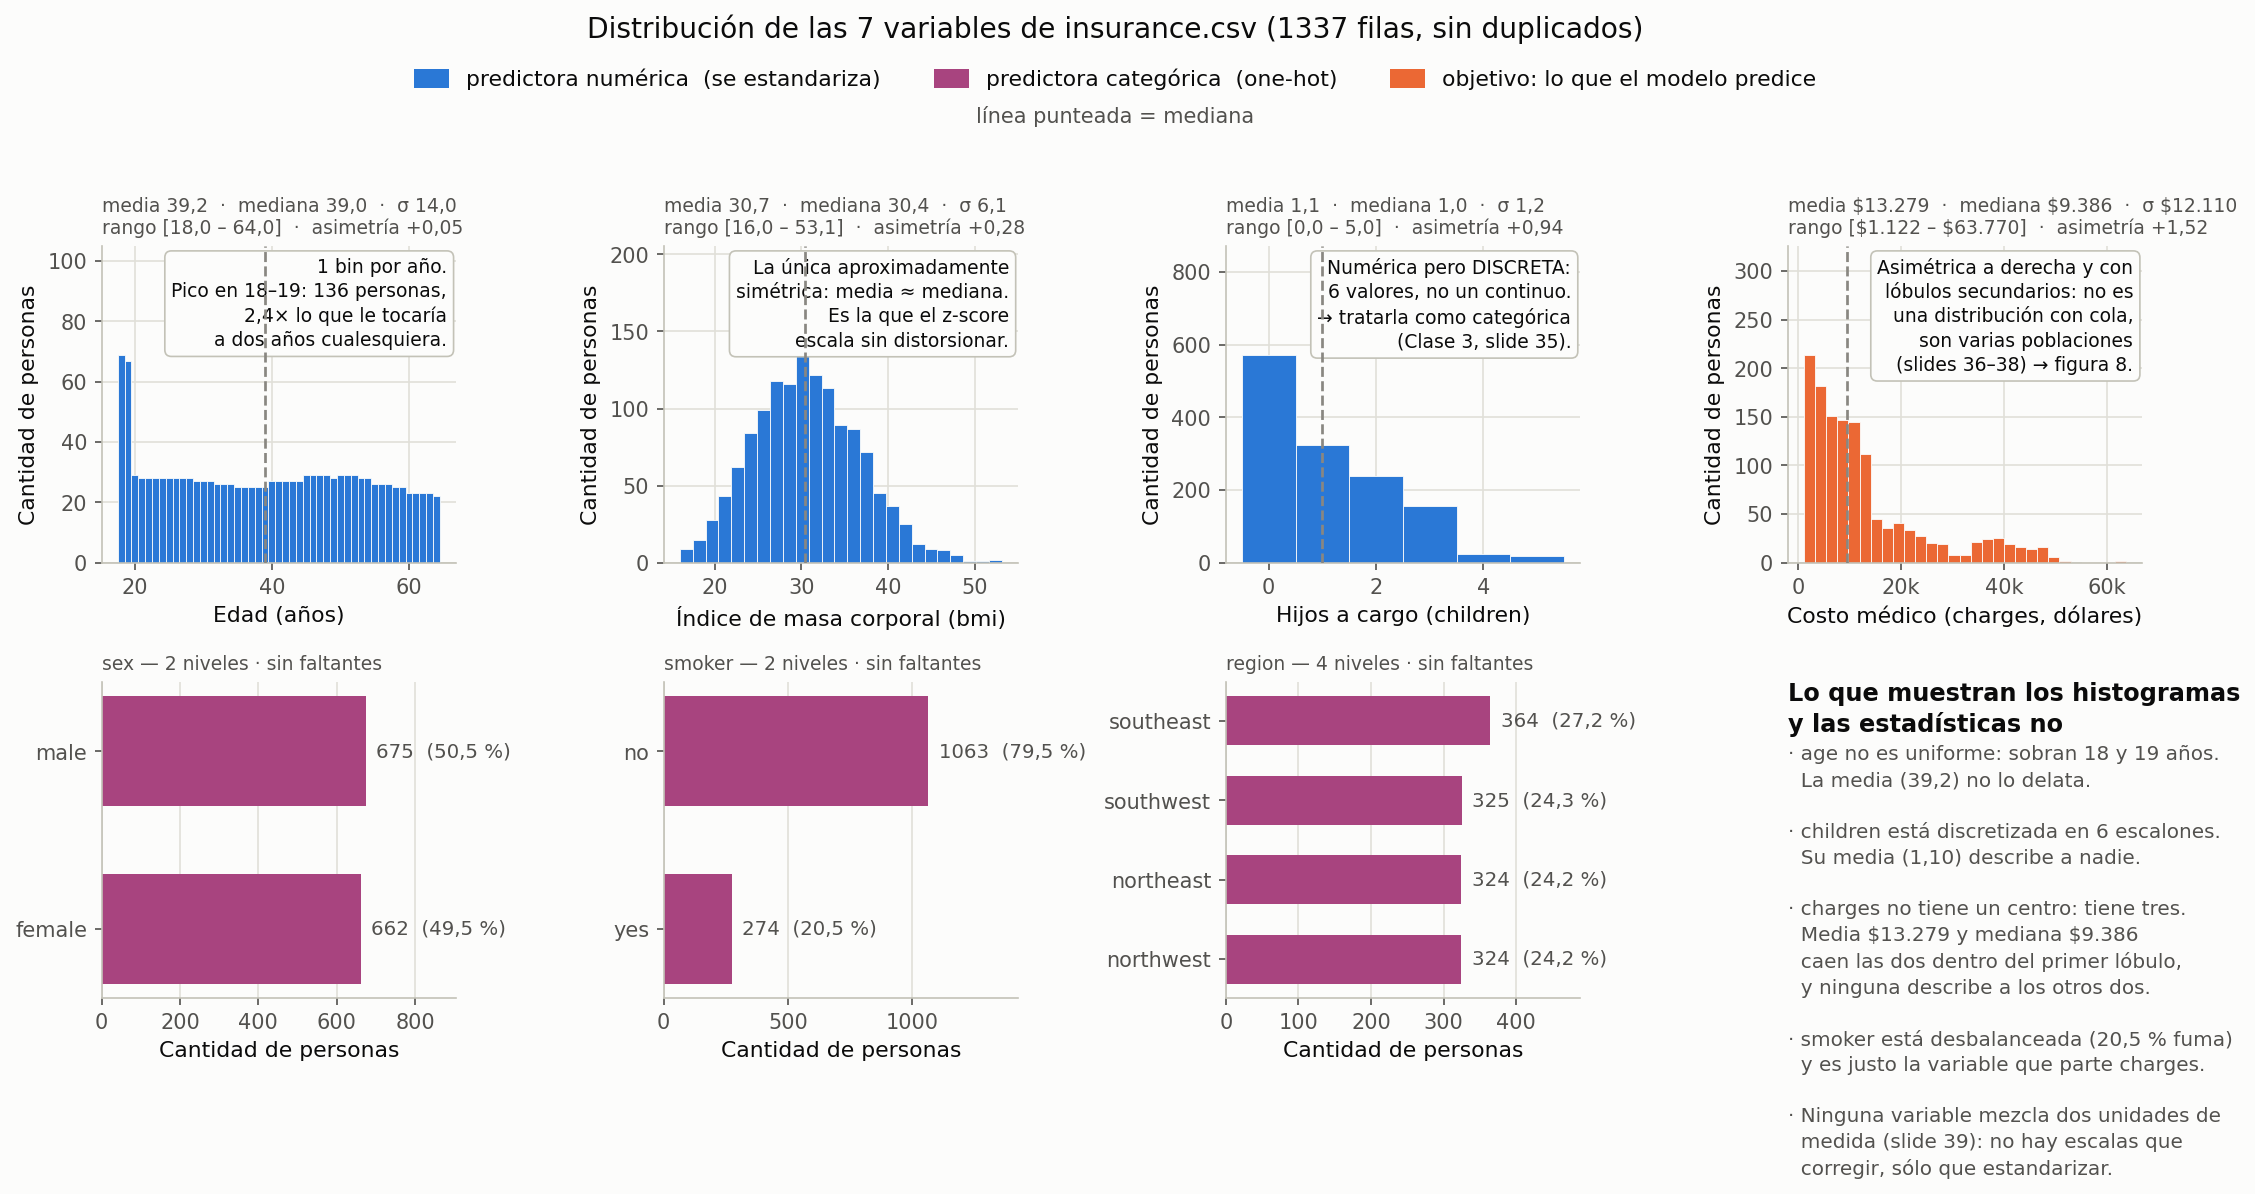
\includegraphics[width=\textwidth]{07-histogramas.png}
\caption{Las siete variables. Arriba las cuatro numéricas, con histograma; abajo las tres
categóricas, con frecuencias. El color codifica el rol de cada variable en el modelo. Las
numéricas enteras (\texttt{age}, \texttt{children}) van con un bin por valor; las continuas
(\texttt{bmi}, \texttt{charges}), con el ancho que da la regla de Freedman--Diaconis, que se
apoya en el rango intercuartil y por lo tanto no se deja inflar por la cola de
\texttt{charges}.}
\label{fig:histogramas}
\end{figure}

Tres cosas aparecen ahí que ninguna tabla de medias muestra, y cada una tiene su análogo
literal en los ejemplos del deck:

\begin{itemize}
  \item \textbf{\texttt{age} no es uniforme.} Hay 136 personas de 18 y 19 años, unas
        2{,}4 veces lo que le tocaría a dos años cualesquiera. La media (39{,}2) no lo delata.
  \item \textbf{\texttt{children} es discreta, no continua}: seis escalones enteros. Es el caso
        del slide 35 ---una variable que parecía continua y el histograma revela discretizada---
        cuya receta es tratarla como categórica. Se evaluó y se descartó; ver D-25.
  \item \textbf{\texttt{charges} no tiene un centro: tiene tres.} Asimetría $+1{,}52$ y lóbulos
        secundarios claros. Es el caso de los slides 36--38, y es el que cambió el modelo de
        este trabajo: se desarrolla en la sección siguiente.
\end{itemize}

Lo que \emph{no} aparece también es resultado: ninguna variable muestra dos escalas superpuestas,
así que no hay unidades de medida mezcladas que corregir (slide 39) ---sólo escalas distintas
que estandarizar, que es otra cosa y se trata más abajo.

\subsection{Variables categóricas}

El dataset tiene tres variables categóricas: \texttt{sex} (binaria), \texttt{smoker} (binaria)
y \texttt{region} (cuatro categorías: \emph{northeast}, \emph{northwest}, \emph{southeast},
\emph{southwest}). Se codificaron con \textbf{one-hot} y no con codificación ordinal porque
esta última le impone al modelo un orden y una distancia numérica que no existen en los datos:
asignar $0,1,2,3$ a las regiones le estaría diciendo que \emph{southwest} está más lejos de
\emph{northeast} que de \emph{southeast} en algún sentido matemático, cuando la variable es
puramente nominal.

Para \texttt{region} se generaron 4 dummies pero se \textbf{descartó una columna}, que queda
como categoría de referencia absorbida en la ordenada al origen. Es la forma estándar de evitar
la \emph{dummy variable trap}: si las 4 dummies estuvieran todas presentes sumarían siempre 1,
lo cual las hace linealmente dependientes de la columna constante del modelo y vuelve singular
la matriz de diseño, de modo que $X^{T}X$ no se puede invertir para resolver por mínimos
cuadrados.

Para las binarias alcanza con \textbf{una sola columna} (\texttt{sex=male},
\texttt{smoker=yes}) en lugar de dos: la segunda categoría es exactamente el complemento de la
primera, así que agregarla sería la misma trampa de colinealidad, sólo que con dos categorías
en vez de cuatro.

El codificador resultante produce 11 columnas: \texttt{age}, \texttt{bmi}, \texttt{children},
\texttt{fumador\_obeso}, \texttt{edad\_al\_cuadrado}, \texttt{bmi\_si\_fuma}, \texttt{sex=male},
\texttt{smoker=yes}, \texttt{region=northwest}, \texttt{region=southeast},
\texttt{region=southwest}.

\subsection{Datos faltantes}

El dataset no tiene ningún valor nulo en las $1338 \times 7$ celdas originales. Sí apareció
\textbf{una fila duplicada exacta} --- los índices 195 y 581 son idénticos en las 7 columnas ---
que se eliminó, quedando 1337 filas.

La eliminación se hace \textbf{antes del split} train/test, y el motivo no es cosmético: un
duplicado exacto repartido entre ambos conjuntos ---una copia en train y la otra en test---
filtraría información del test hacia el entrenamiento sin que el modelo tuviera que generalizar
nada. El error de test quedaría artificialmente bajo para esa fila.

\subsection{Outliers}

Se comparó la detección por \textbf{rango intercuartílico (IQR)} contra \textbf{z-score}, y se
optó por IQR. La tabla de discrepancia muestra por qué:

\begin{table}[H]
\centering
\caption{Los dos criterios no coinciden, y la discrepancia se explica.}
\begin{tabular}{lrr}
\toprule
\textbf{Variable} & \textbf{IQR detecta} & \textbf{Z-score detecta} \\
\midrule
\texttt{charges}  & 139 (10,4\,\%) & 7 \\
\texttt{children} & 0              & 18 \\
\bottomrule
\end{tabular}
\end{table}

En \texttt{charges}, el z-score detecta muchísimo menos porque su propia definición depende de
la media y el desvío estándar, y \texttt{charges} tiene una asimetría de $1{,}516$: los valores
extremos ---que son justamente los que se querría detectar--- arrastran la media hacia arriba e
\textbf{inflan el desvío estándar}, con lo cual ``tres desvíos de la media'' deja de ser un
umbral exigente. Los propios outliers se disfrazan a sí mismos. El IQR, al basarse en
cuartiles, es robusto a esa distorsión.

En \texttt{children} pasa lo inverso: el z-score marca 18 valores y el IQR ninguno, porque
\texttt{children} es un entero acotado entre 0 y 5, y ``estar a tres desvíos de la media'' no
significa lo mismo en una variable discreta de rango chico que en una continua sin cota.

\paragraph{Los outliers se conservan.}
De los 139 outliers de \texttt{charges} detectados por IQR, el \textbf{97,8\,\% son fumadores},
contra apenas 11,5\,\% de fumadores en el resto de la población. Esa desproporción es la
evidencia de que \textbf{no son errores de carga, son una subpoblación real}: fumar dispara el
costo médico de forma no lineal, y esos 139 casos son la cola derecha esperable de esa
subpoblación, no ruido. Eliminarlos le escondería al modelo justo el fenómeno más importante
del dataset.

\begin{figure}[H]
\centering
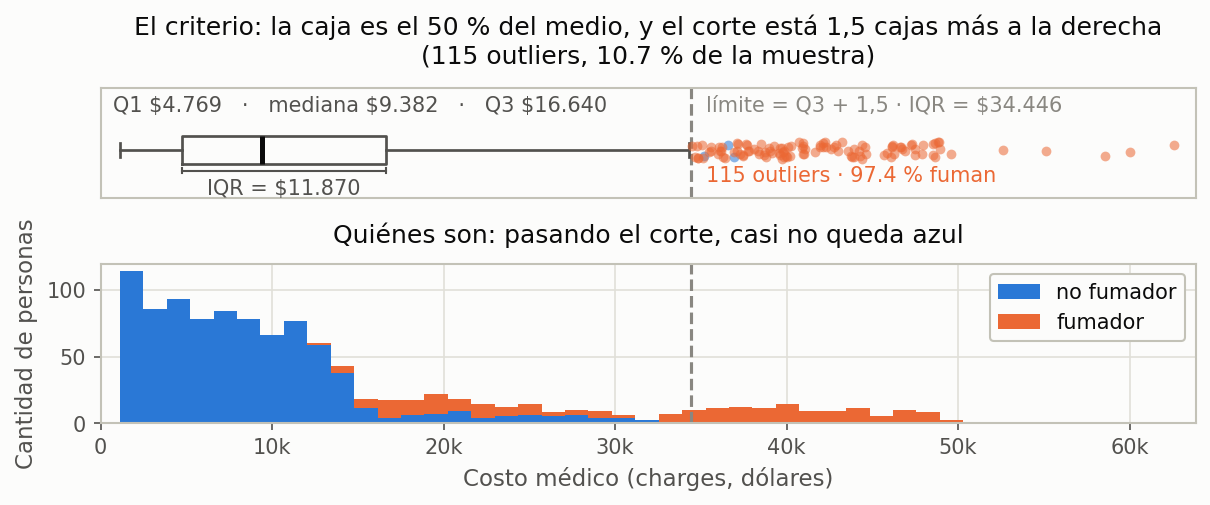
\includegraphics[width=\textwidth]{04-outliers-charges.png}
\caption{Arriba: de dónde sale el criterio. La caja va de $Q_1$ a $Q_3$ ---el 50\,\% central---
y su ancho es el IQR; el corte está una caja y media más a la derecha. Abajo: quiénes quedan de
ese lado, con la misma distribución apilada por condición de fumador. Los dos paneles comparten
el eje horizontal, así que el umbral punteado es una sola vertical que los cruza. La cola larga
por encima del corte es \emph{casi enteramente} de fumadores (97,8\,\%), que es el argumento para
conservarla.}
\end{figure}

\subsection{Las tres poblaciones de \texttt{charges}, y la característica que salió de ahí}
\label{sec:poblaciones}

El histograma de \texttt{charges} muestra un pico grande y dos jorobas a la derecha. La Clase 3
no se queda en constatarlo: cuando aparece un segundo pico, prescribe (a) darle esa información
al sistema como variable binaria o (b) partir el dataset y entrenar dos modelos, y antes de
decidir, «ver el histograma separado para cada población para ver si realmente son distintas».
La figura~\ref{fig:poblaciones} es ese paso.

\begin{figure}[H]
\centering
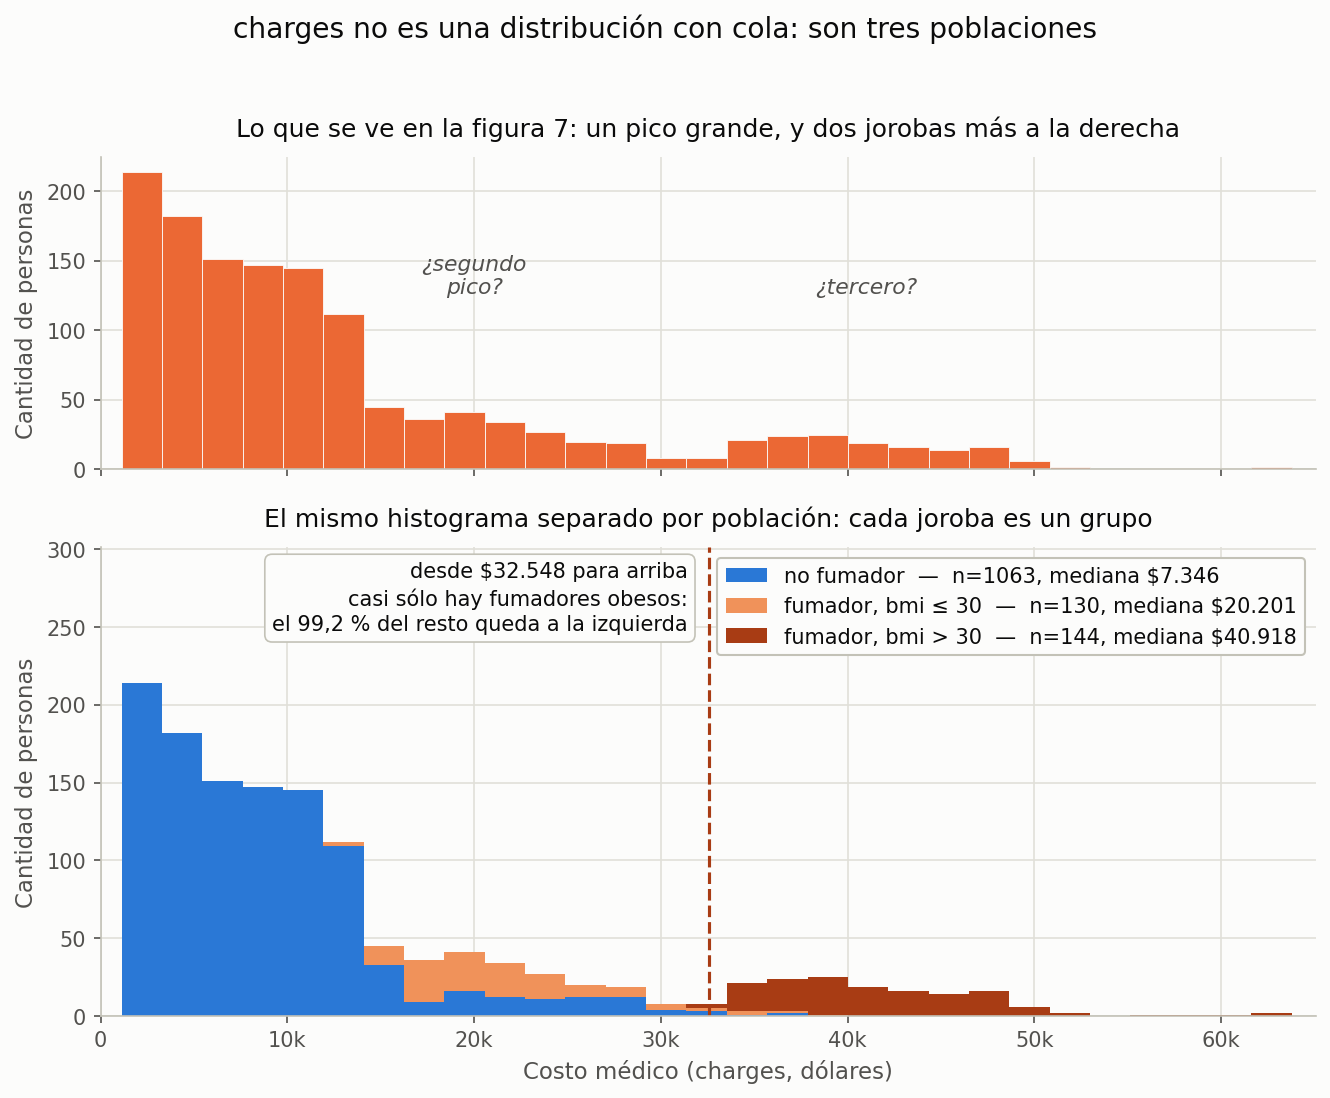
\includegraphics[width=0.88\textwidth]{08-charges-poblaciones.png}
\caption{Arriba, \texttt{charges} sin separar. Abajo, el mismo histograma con los mismos bins,
partido por población. Las medianas son \$7.346, \$20.201 y \$40.918.}
\label{fig:poblaciones}
\end{figure}

Son tres, y no se separan igual de bien. El grupo de fumadores con bmi $\leq 30$ se solapa con
la cola de los no fumadores; el de fumadores con bmi $> 30$ arranca en \$32.548, por encima del
99{,}2\,\% de todos los demás.

\paragraph{Es un escalón, no una pendiente.} La distinción decide qué hacer. Partiendo el bmi en
tramos finos alrededor de 30, entre los fumadores el costo medio salta de \$23.555 en el tramo
$[29,30)$ a \$38.799 en el $[30,31)$ ---unos quince mil dólares en una unidad de bmi---, con
pendiente suave a los dos lados del corte; entre los no fumadores el mismo corte casi no mueve
nada (\$8.257 contra \$8.058). Si fuera una pendiente, los saltos entre tramos contiguos serían
todos parecidos.

Eso importa porque la expansión polinómica de grado 2 \emph{ya} genera el término
\texttt{bmi*smoker=yes}, y el modelo lo conserva con peso $+3.317$. Pero un producto con una
variable continua sólo puede representar un cambio de pendiente: no puede representar un salto.
Por eso se agrega la característica binaria
\[
  \texttt{fumador\_obeso} \;=\; (\texttt{smoker}=\text{yes}) \;\wedge\; (\texttt{bmi} > 30),
\]
que es la opción (a) del deck (decisión D-23). El umbral 30 es el de la OMS: es una constante
médica, externa a este dataset, y esa procedencia es lo que hace legítimo usarla ---no sale de
buscar cuál corte minimiza el error. El barrido de umbrales lo confirma igual: el mínimo cae
exactamente en 30, con 29 y 31 claramente peores.

No es fuga de datos: las dos columnas de las que sale están disponibles al momento de predecir y
\texttt{charges} no interviene en el cálculo. Y el efecto es de la \emph{interacción}, no de sus
partes: agregar sólo \texttt{bmi} $>30$ deja el error prácticamente donde estaba.

\subsection{Características y escalado}

El enunciado pide dos decisiones justificadas, y van por separado.

\paragraph{Qué características se incluyen: las seis originales, sin descartar ninguna, más dos
derivadas.}
El enunciado admite explícitamente que ``pueden ser todas'', y en este dataset esa es además la
respuesta correcta para las seis variables crudas. A ellas se suman \texttt{edad\_al\_cuadrado}
(D-27) y \texttt{bmi\_si\_fuma} (D-28), que la tabla documenta junto con las demás porque son la
otra mitad de esta misma decisión: no alcanza con no tirar nada, también hay que agregar lo que
la estructura del dataset pide (\texttt{fumador\_obeso} ya se presentó en la
sección~\ref{sec:poblaciones} con la misma lógica):

\begin{table}[H]
\centering
\caption{Decisión de inclusión, variable por variable.}
\begin{tabular}{@{}l l p{9.2cm}@{}}
\toprule
\textbf{Variable} & \textbf{¿Se incluye?} & \textbf{Por qué} \\
\midrule
\texttt{age}      & Sí & Segunda correlación más alta con \texttt{charges} ($0{,}299$) y relación monótona clara. En el modelo de producción queda con coeficiente $45{,}10$. \\
\texttt{bmi}      & Sí & Correlación baja ($0{,}198$) pero no descartable: su efecto depende de \texttt{smoker}, y Pearson mide relación lineal, no interacciones. Coeficiente $111{,}20$. \\
\texttt{children} & Sí & Correlación $0{,}068$, la más débil. Se conserva igual: es barata, y en el modelo de producción (lineal, sin regularizar) queda con coeficiente $815{,}02$. \\
\texttt{sex}      & Sí & Binaria, una columna. El modelo de producción no regulariza, así que no hay penalización que la apague: queda con coeficiente $-218{,}32$ (\texttt{sex=male}), de los más chicos en magnitud entre los once, pero no nulo. \\
\texttt{smoker}   & Sí & La variable más informativa del dataset (correlación $0{,}787$). \\
\texttt{region}   & Sí & Tres columnas tras el one-hot. Aporta poco, pero es la única variable geográfica y su costo es mínimo. \\
\texttt{edad\_al\_cuadrado} & Sí & Derivada (D-27): captura la \emph{curvatura} del costo con la edad, que un término lineal en \texttt{age} no puede representar. Coeficiente $3749{,}13$, el tercero más grande de los once. \\
\texttt{bmi\_si\_fuma} & Sí & Derivada (D-28): captura la \emph{pendiente} del bmi, distinta entre fumadores y no fumadores. Coeficiente $5236{,}99$, el más grande de los once. \\
\bottomrule
\end{tabular}
\end{table}

\paragraph{Advertencia de interpretabilidad.} Agregar \texttt{edad\_al\_cuadrado} y
\texttt{bmi\_si\_fuma} tiene un costo. \texttt{edad\_al\_cuadrado} es, literalmente, una función
determinista de \texttt{age}, y \texttt{bmi\_si\_fuma} lo es de \texttt{bmi} dentro del grupo de
fumadores: están muy correlacionadas entre sí. Por eso los coeficientes de \texttt{age} y
\texttt{bmi} cayeron tan fuerte respecto de la versión anterior del pipeline (\texttt{age}: de
$3754$ a $45{,}10$; \texttt{bmi}: de $333$ a $111{,}20$), y el de \texttt{smoker=yes} también bajó
(de $5437$ a $1161{,}22$): las derivadas absorbieron buena parte del efecto que antes cargaba la
variable original. Eso no significa que \texttt{age} o \texttt{bmi} dejaron de importar --- significa
que, dentro de cada grupo (\texttt{age} con \texttt{edad\_al\_cuadrado}; \texttt{bmi},
\texttt{smoker=yes} y \texttt{fumador\_obeso} con \texttt{bmi\_si\_fuma}), los coeficientes
individuales ya no son interpretables por separado: sólo tiene sentido leerlos como grupo. Es un
costo real de interpretabilidad a cambio de mejor ajuste.

El criterio general es que \textbf{no se descarta ninguna variable a mano}. Con 1337 filas y
sólo 11 columnas tras codificar no hay problema de dimensionalidad que lo justifique, y sacar
una variable mirando su correlación con el objetivo es una decisión tomada \emph{con los
datos}, exactamente el tipo de elección que después contamina la evaluación. La selección de
variables se delega a la penalización $L_1$, que la hace \textbf{dentro de cada fold} y por lo
tanto sin fuga.

\paragraph{El escalado.}
Las variables numéricas se \textbf{estandarizan} (media 0, desvío 1) antes de ajustar cualquier
modelo con regularización, porque Lasso penaliza la magnitud de los coeficientes: si las
variables están en escalas distintas ---\texttt{age} en años, \texttt{bmi} en kg/m$^2$,
\texttt{children} en unidades enteras chicas--- la penalización castiga más a los coeficientes
de las variables que naturalmente necesitan valores grandes, sin que eso tenga que ver con su
importancia real.

El punto crítico es \textbf{cuándo} se calculan la media y el desvío: \textbf{siempre sobre el
fold de entrenamiento únicamente}, nunca incluyendo el fold de validación. Es la misma lógica
que con el test. Si se calcularan sobre todos los datos, la validación dejaría de ser una
medición honesta, porque el escalado ya habría ``visto'' esos datos antes de que el modelo
intentara predecirlos.

% =====================================================================
\section{Puntos 2 y 3 --- Implementación}
% =====================================================================

\subsection{El pipeline, de punta a punta}

\begin{enumerate}
  \item \texttt{quitar\_duplicados}: $1338 \rightarrow 1337$ filas.
  \item \texttt{agregar\_derivadas}: agrega tres columnas ---\texttt{fumador\_obeso} (D-23),
        \texttt{edad\_al\_cuadrado} (D-27) y \texttt{bmi\_si\_fuma} (D-28)---. Ocurre
        \textbf{antes del split}, porque las columnas de las que salen ya están disponibles
        para cualquier fila y ninguna usa \texttt{charges}.
  \item \texttt{separar\_train\_test} con semilla 42: 1070 filas de train, 267 de test (80/20).
  \item \texttt{CodificadorCategoricas}, ajustado \textbf{sólo con train}: produce las 11
        columnas descriptas arriba.
  \item \texttt{k\_fold}: partición propia en 5 folds sobre el train.
  \item Dentro de cada fold: \texttt{Estandarizador} (ajustado sólo con el fold de
        entrenamiento) $\rightarrow$ \texttt{expandir\_polinomica} $\rightarrow$
        \texttt{Estandarizador} otra vez $\rightarrow$ ajuste del modelo.
  \item Modelos: \texttt{RegresionLineal} (mínimos cuadrados vía descomposición en valores
        singulares) y \texttt{Lasso} (descenso por coordenadas con actualización incremental
        del residuo).
\end{enumerate}

\subsection{Cómo se separaron train y test, y por qué así}

El procedimiento concreto es: se genera una \textbf{permutación aleatoria} de los índices
$0\ldots1336$ y se corta, mandando las últimas $\mathrm{round}(1337 \times 0{,}2) = 267$
posiciones a test y las 1070 restantes a train. Tres decisiones dentro de eso:

\begin{itemize}
  \item \textbf{Se baraja antes de cortar.} Tomar las últimas 267 filas del archivo tal como
        viene sería válido sólo si el orden fuera aleatorio, y eso no se puede dar por sentado:
        los CSV suelen venir ordenados por algún criterio. Barajar rompe cualquier estructura
        latente en el orden.
  \item \textbf{La semilla es fija (42).} Sin semilla fija ningún número de este informe sería
        reproducible. También evita una trampa sutil: si la semilla variara, sería posible
        correr varias veces y quedarse con la partición que da mejores números, que es una
        forma encubierta de ajustar contra el test.
  \item \textbf{No se estratifica ---y el motivo cambió (D-24).} La versión previa de este
        informe decía que no hay clases que preservar porque el objetivo es continuo. El
        análisis exploratorio de la Clase 3 lo refuta: \texttt{charges} no es una distribución
        continua unimodal sino \emph{tres poblaciones casi disjuntas} (figura~\ref{fig:poblaciones}),
        y los cinco folds reparten la tercera de forma desigual ---entre 17 y 31 personas, del
        7{,}9\,\% al 14{,}5\,\%---, con correlación $+0{,}62$ entre esa proporción y el
        \texttt{charges} medio del fold. Hay clases de facto, y se reparten mal.

        Lo que ocurre es que estratificar por ellas \emph{no cambia nada}, y eso se midió:
        promediando sobre ocho particiones, el desvío del RMSE entre folds es 593 con folds
        aleatorios y 591 con folds estratificados ---dos dólares, cuando entre dos particiones
        del mismo método la diferencia va de 410 a 715---. Lo que mueve el error de un fold no
        es cuántos fumadores obesos le tocaron sino cuáles: dentro de ese grupo los costos van
        de \$32.548 a \$63.770 (sobre el dataset completo, como todo el EDA del punto 1), así que
        igualar los conteos deja intacta la varianza que
        importa. La estratificación controla justo la dimensión que no era el problema. La
        decisión se sostiene; su justificación es ahora una medición y no una definición
        equivocada.

  \item \textbf{Sí sigue valiendo el resto.} No hay estructura temporal ni de grupos ---cada
        fila es una persona distinta--- así que el supuesto de independencia que justifica el
        barajado se cumple.
\end{itemize}

\subsection{La regresión polinómica sigue siendo lineal en los parámetros}

Elevar \texttt{age} al cuadrado o multiplicar \texttt{bmi} por \texttt{smoker=yes} no cambia la
naturaleza del modelo: sigue siendo una combinación lineal de columnas de la matriz de diseño,
sólo que esas columnas ahora son transformaciones no lineales de las variables originales. Lo
que se ajusta por mínimos cuadrados es exactamente el mismo problema que con grado 1; lo único
que cambia es qué características se le presentan al modelo.

\subsection{Regularización $L_1$}

El objetivo que minimiza el Lasso implementado es
\begin{equation}
J(w) \;=\; \frac{1}{2n}\,\lVert y - Xw - b \rVert_2^{2} \;+\; \lambda\,\lVert w \rVert_1 ,
\end{equation}
resuelto por descenso por coordenadas con \emph{soft-thresholding}. El intercepto $b$ no se
penaliza: se obtiene centrando $X$ e $y$ y recuperándolo como
$b = \bar{y} - \bar{x}^{T} w$. Penalizarlo encogería la predicción media hacia cero, que no es
lo que la regularización busca.

La grilla de $\lambda$ se construye \textbf{relativa a} $\lambda_{\max}$, el menor valor que
anula todos los coeficientes:
\begin{equation}
\lambda_{\max} \;=\; \max_{j}\;\frac{\lvert x_j^{T}(y - \bar{y}) \rvert}{n} .
\end{equation}
Ese máximo se calcula sobre el train completo, y da $10360{,}94$ ---el mismo valor para los
grados 2, 3 y 4---. Una grilla relativa es interpretable y comparable entre grados; una absoluta
elegida a ojo, no.

% =====================================================================
\section{Punto 4 --- Resultados}
% =====================================================================

\begin{table}[H]
\centering
\caption{Validación cruzada de 5 folds sobre las 1070 filas de entrenamiento. Regresión lineal
sin regularizar, por grado del polinomio. Tabla generada por \texttt{src/tablas.py} a partir de
\texttt{resultados/cv\_lineal.csv}.}
\tablacvlineal
\end{table}

\begin{table}[H]
\centering
\caption{Lasso, mismo esquema de validación cruzada. Las configuraciones que no
convergieron quedan excluidas de la selección (D-20). Tabla generada por
\texttt{src/tablas.py} a partir de \texttt{resultados/cv\_lasso.csv}.}
\tablacvlasso
\end{table}

\subsection{Dónde está el sobreajuste, y cómo se lo reconoce}

\begin{figure}[H]
\centering
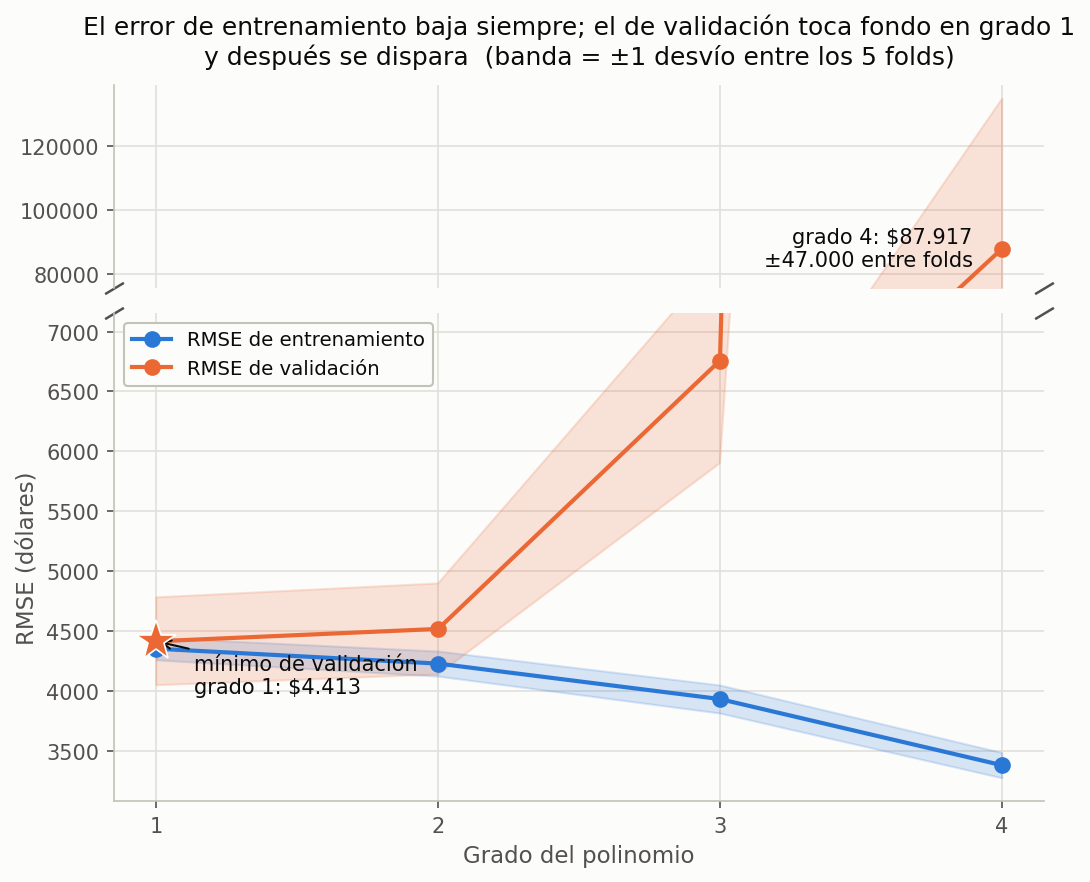
\includegraphics[width=0.92\textwidth]{01-curvas-train-val.png}
\caption{El error de entrenamiento baja monótonamente con el grado; el de validación toca
fondo en grado 1 y después sube, hasta dispararse en grado 4. El eje está \emph{partido}: el
grado 4 se va a 87.916,9 dólares y en una escala única aplastaría a los otros tres hasta
volverlos ilegibles. La banda es $\pm 1$ desvío entre folds.}
\label{fig:curvau}
\end{figure}

En regresión lineal sin regularizar el sobreajuste empieza ya en grado 2 y se vuelve catastrófico
en grado 4. El error de \textbf{train} baja monótonamente ($4351{,}6 \rightarrow 4227{,}2
\rightarrow 3931{,}1 \rightarrow 3379{,}1$ dólares), porque más características siempre le dan
al modelo más grados de libertad para ajustar lo que ya vio. El de \textbf{validación} hace
exactamente lo contrario desde el arranque: toca su mínimo en grado 1 ($4413{,}4$) y sube en
cada grado siguiente, hasta $87916{,}9$ en grado 4 ---\textbf{19,9 veces} el del grado 1---.

\paragraph{Por qué el grado 4 se dispara así.} No es sólo que sobreajuste: es que el problema
deja de estar determinado. La expansión de grado 4 sobre once características da
\textbf{1364 columnas}, y el diagnóstico de rango que corre \texttt{src/experimentos.py} muestra que su
rango efectivo es 436: el \textbf{68,0\,\%} de las columnas son combinación lineal exacta de las
otras (las causas están en \emph{Limitaciones}). Una de esas causas es nueva desde que se
agregaron \texttt{edad\_al\_cuadrado} y \texttt{bmi\_si\_fuma}: a partir de grado 2 la propia
expansión polinómica las \textbf{duplica exactamente} ---\texttt{age}$\times$\texttt{age} vuelve
a calcular \texttt{edad\_al\_cuadrado}, y \texttt{bmi}$\times$\texttt{smoker=yes} vuelve a
calcular \texttt{bmi\_si\_fuma}---, y esa duplicación es buena parte de por qué la redundancia
sube al 68\,\% y por qué esta vez son \textbf{cuatro} las configuraciones que no convergen, no
dos. En grado 1, que es el de producción, la duplicación no existe: cada característica aparece
una sola vez. Con
856 filas por fold de entrenamiento, el ajuste de mínimos cuadrados sobre ese espacio es una
extrapolación, y lo que predice fuera del fold no tiene por qué parecerse a nada.

El indicador más claro de sobreajuste no es sólo que el RMSE de validación suba, sino que la
\textbf{brecha} entre train y validación crezca sistemáticamente: de \destacado{61,8 dólares} en
grado 1 a \destacado{84.537,9 dólares} en grado 4. Un modelo que generaliza bien tiene un error de
validación parecido al de train; una brecha que se ensancha es la firma directa de que el
modelo está aprendiendo particularidades del fold de entrenamiento que no se sostienen fuera.

El segundo indicador, más sutil pero igual de contundente, es la \textbf{estabilidad entre
folds}: el desvío del RMSE de validación pasa de $\pm 367{,}0$ en grado 1 a $\pm 47.000{,}1$ en
grado 4, \textbf{128 veces más grande}. Eso dice algo distinto de ``el modelo es peor en
promedio'': dice que el modelo de grado 4 es \textbf{inestable}, que su desempeño cambia
drásticamente según qué filas caen en cada partición.

\paragraph{Una observación sobre el desvío en grado 1.} Los $\pm 367{,}0$ del modelo elegido son
más altos que los $\pm 355{,}3$ que daba el mismo grado 1 antes de D-23, y eso no es un defecto:
es la contracara del hallazgo. Al capturar el escalón de \texttt{fumador\_obeso}, el modelo
elimina el error sistemático que dominaba antes, y lo que queda es el error idiosincrásico de
los casos extremos ---cuya repartición entre folds es justamente lo que varía---. Es el mismo
fenómeno que explica por qué estratificar no ayuda (D-24).

\begin{figure}[H]
\centering
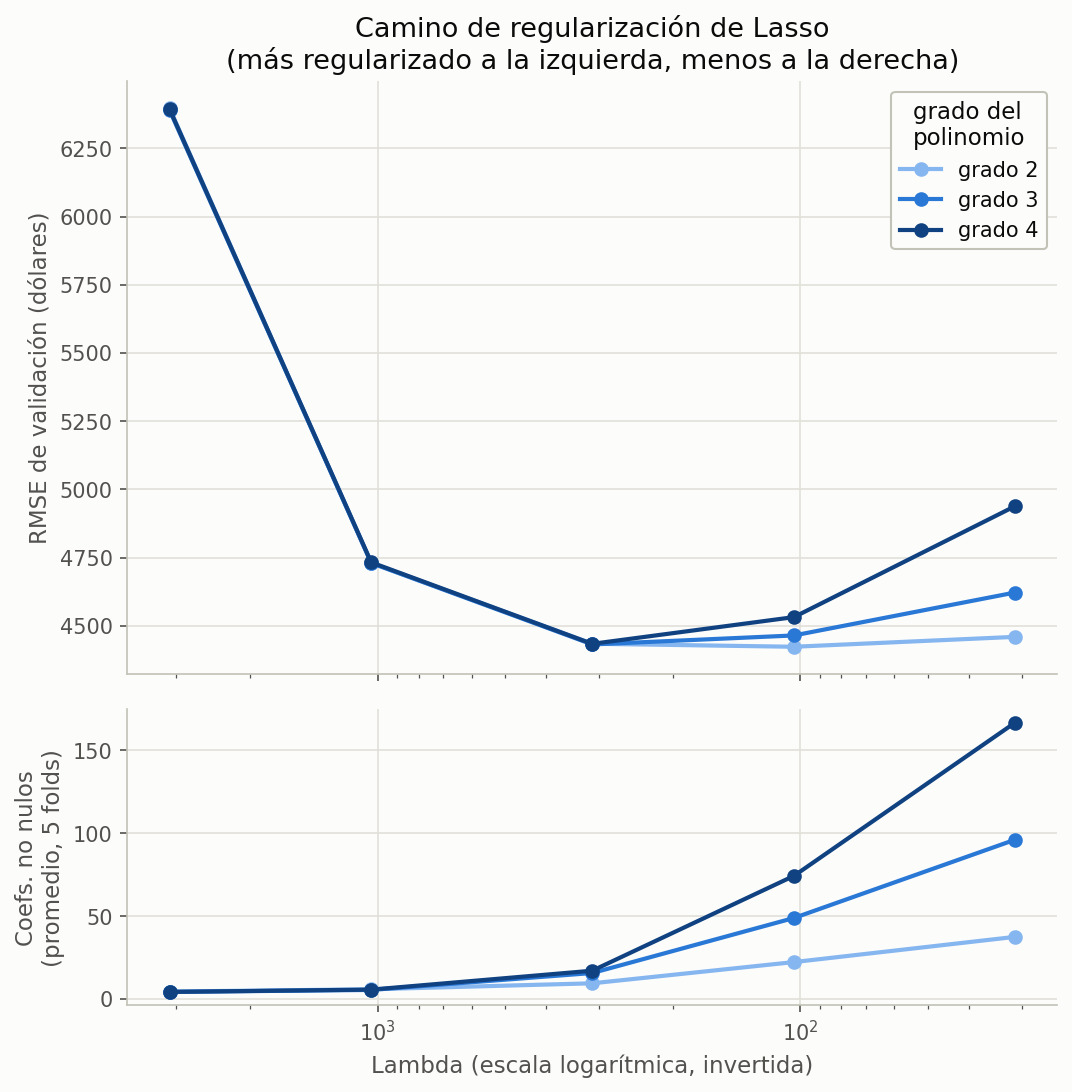
\includegraphics[width=0.78\textwidth]{02-camino-lasso.png}
\caption{Camino de regularización. Al aflojar $\lambda$ entran más características (panel
inferior) y el error primero baja y después vuelve a subir. El tono codifica el grado del
polinomio: más oscuro, grado más alto.}
\end{figure}

Lasso corrige el problema en buena medida: el mejor $\lambda$ de grado 4 que efectivamente
converge ($\lambda = 310{,}83$) lleva el RMSE de validación de $87916{,}9$ a $4433{,}7$ dólares
---prácticamente las mismas 19,9 veces de distancia que separan al grado 4 sin regularizar del
grado 1, pero recorridas en el sentido contrario--- dejando vivos 17,0 de los 1364 coeficientes
en promedio. Que la penalización $L_1$ recupere de un espacio degenerado un error comparable al
del modelo lineal simple es exactamente lo que la regularización promete, y acá se ve en su
forma más extrema.

Lo que \emph{no} logra es superarlo: el mejor Lasso de toda la tabla (grado 2, $\lambda =
103{,}61$) queda en $4422{,}92$, apenas nueve dólares por encima del lineal de grado 1, con 22,2
características vivas en promedio en lugar de 11. Sobre esa comparación decide el punto
siguiente.

% =====================================================================
\section{Punto 5 --- Las tres respuestas}
% =====================================================================

\subsection{¿Qué modelo obtuvo menor error?}

El de menor RMSE de validación cruzada es, directamente, \textbf{la regresión lineal de grado 1
sin regularizar}: RMSE de validación $= 4413{,}45 \pm 366{,}97$, con las once características de
grado 1, todas vivas. El mejor Lasso de toda la búsqueda (grado 2, $\lambda = 103{,}61$) queda
apenas nueve dólares por encima, en $4422{,}92$, con 22,2 coeficientes vivos en promedio.

\subsection{¿Cuál se implementaría en una aplicación real?}

\textbf{El mismo modelo que ganó la sección anterior}, y esta vez la pregunta se responde sola:
no hay que elegir entre el de menor error y el más simple porque son la misma configuración.

De todos modos vale correr el procedimiento completo, para no decidir por comodidad. Aplicando
la \textbf{regla de 1 error estándar} sobre el ganador,
\begin{equation}
\mathrm{ES} \;=\; \frac{366{,}97}{\sqrt{5}} \;=\; 164{,}11 ,
\qquad
\text{umbral} \;=\; 4413{,}45 + 164{,}11 \;=\; 4577{,}56 ,
\end{equation}
de las 19 configuraciones corridas, \textbf{cuatro} no convergieron y quedan fuera de la
comparación (D-20): Lasso de grado 3 con $\lambda = 310{,}83$, $\lambda = 103{,}61$ y
$\lambda = 31{,}08$, y Lasso de grado 4 con $\lambda = 31{,}08$. Sobre las 15 configuraciones
elegibles que quedan, \destacado{7 caen por debajo del umbral}. Esas 7 son, para los datos
disponibles, \textbf{indistinguibles entre sí}: cuál aparece primera en la tabla depende del azar
de cómo cayó la partición en 5 folds, no de una diferencia real de capacidad predictiva.

Frente a un empate estadístico, lo habitual sería resolver por la configuración \textbf{más
simple} del grupo empatado. Ese paso, esta vez, es innecesario: la más simple de las 7 ---once
características, grado 1, sin regularizar, sin ningún hiperparámetro que ajustar, y por lejos la
de menos columnas en la matriz de diseño--- \textbf{ya es} la que tiene el menor error de
validación cruzada de toda la búsqueda. La regla de 1 ES no decide nada acá: sólo
\textbf{confirma} lo que el mínimo ya decía. Y como ganador de la CV y modelo de producción son,
por primera vez, el mismo modelo, el costo de la simplicidad es \destacado{\costosimplicidad
dólares}: no hay nada que sacrificar a cambio de un modelo más simple.

Vale subrayar lo que eso significa, porque es el resultado central del trabajo: \emph{con las
características correctas, ni la expansión polinómica ni la regularización compran nada}. Las
dos existen para darle al modelo la flexibilidad de representar relaciones que las variables
crudas no representan; una vez que \texttt{fumador\_obeso}, \texttt{edad\_al\_cuadrado} y
\texttt{bmi\_si\_fuma} las representan de forma explícita, la flexibilidad extra sólo agrega
varianza. Antes de D-23 el mismo procedimiento elegía Lasso de grado 2 con 44 características,
porque sin esas columnas derivadas el modelo lineal \emph{sí} se quedaba corto (6122{,}8 de RMSE
de validación).

\begin{table}[H]
\centering
\caption{Historia del RMSE de test a medida que el pipeline sumó características derivadas.
Desde D-27/D-28, ganador de la CV y modelo de producción son el mismo modelo: no hay una fila
separada que reportar para cada uno. Las dos filas intermedias son registro de los pipelines
anteriores, verificable y no una afirmación (D-26).}
\begin{tabular}{lrrr}
\toprule
\textbf{Modelo} & \textbf{Características} & \textbf{Coefs. vivos} & \textbf{RMSE test} \\
\midrule
\textbf{Producción = ganador de la CV (lineal grado 1)} & \textbf{\featuresproduccion} & \textbf{\coefsproduccion} & $\mathbf{\rmsetestproduccion}$ \\
\midrule
\emph{Producción entre D-23 y D-27/D-28} (lineal grado 1, sin \texttt{edad\_al\_cuadrado} ni \texttt{bmi\_si\_fuma}) & \emph{9} & \emph{9} & \emph{4.465,32} \\
\emph{Producción anterior a D-23} (Lasso grado 2, $\lambda=286{,}4$) & \emph{44} & \emph{10} & \emph{4.739,33} \\
\midrule
Baseline: predecir siempre la media                & --- & 0  & \rmsetestbaseline \\
\bottomrule
\end{tabular}
\end{table}

En tres pasos el RMSE de test bajó de 4.739,33 a 4.465,32 y a \rmsetestproduccion:
\destacado{450,81 dólares menos, un 9,5\,\%} sobre el punto de partida. La primera mejora vino de
\texttt{fumador\_obeso} (D-23); la segunda, de sumar \texttt{edad\_al\_cuadrado} y
\texttt{bmi\_si\_fuma} (D-27, D-28). Ninguna de las dos vino de agregar grados de libertad al
polinomio ni de ajustar un hiperparámetro de regularización: las tres características derivadas
son la mejora completa.

\subsection{¿Qué RMSE se espera en datos nuevos?}

\begin{center}
\fbox{\parbox{0.85\textwidth}{\centering\vspace{2pt}
\textbf{\rmsetestproduccion dólares} --- el RMSE de \textbf{test} del modelo de producción,\\
\textbf{no} su RMSE de validación (\rmsevalproduccion).\vspace{2pt}}}
\end{center}

Es importante entender por qué el número de validación está sesgado a la baja y no se puede
prometer. Esa configuración se eligió por tener, directamente, el RMSE de validación \textbf{más
bajo} de las 15 estimaciones elegibles (de 19 corridas; cuatro quedaron fuera por no converger).
Cada una de esas estimaciones tiene ruido de muestreo, porque es un promedio sobre sólo 5 folds.
Cuando se elige el \textbf{mínimo} de un conjunto de estimaciones ruidosas, ese mínimo queda
sesgado hacia abajo \emph{aunque cada estimación individual sea insesgada}: es más probable que
el ``ganador'' lo sea en parte por haber tenido una racha favorable de ruido, no sólo por ser
mejor de verdad. Acá ese argumento aplica de lleno y sin salvedades ---no hay un modelo elegido
por simplicidad y otro que ganó la CV: hay uno solo, y es exactamente el mínimo de la tabla---.
El test, al no haber participado de ninguna decisión, no tiene ese sesgo.

Y sin embargo el test dio \emph{mejor} que la validación: \rmsetestproduccion{} contra
\rmsevalproduccion{}, una diferencia de $-124{,}93$ dólares. Eso no contradice el argumento
anterior: el sesgo de selección predice que el test tienda a ser peor \emph{en promedio}, no que
lo sea en esta partición puntual, y $124{,}93$ dólares es chico frente al $\pm 366{,}97$ de
ruido que ya separaba a los folds entre sí durante la validación. Con una sola partición de test
no hay forma de saber si el ruido jugó a favor esta vez o si el sesgo es de verdad más chico de
lo que la teoría sugiere.

\paragraph{Dos advertencias que corresponde dar junto con ese número.}
\begin{itemize}
  \item El conjunto de test tiene \textbf{267 filas}. El \rmsetestproduccion es en sí mismo una
        estimación con su propia incertidumbre de muestreo, que este trabajo no cuantificó con
        un intervalo de confianza. No hay que leerlo con cuatro decimales.
  \item El RMSE \textbf{promedia sobre una población heterogénea}. El error no se reparte
        parejo: se concentra en los fumadores, que son los casos más caros y los que más le
        importa acertar a una aseguradora. Prometer un único RMSE global oculta esa asimetría.
\end{itemize}

\begin{figure}[H]
\centering
\IfFileExists{../figuras/05-predicho-vs-real.png}{%
  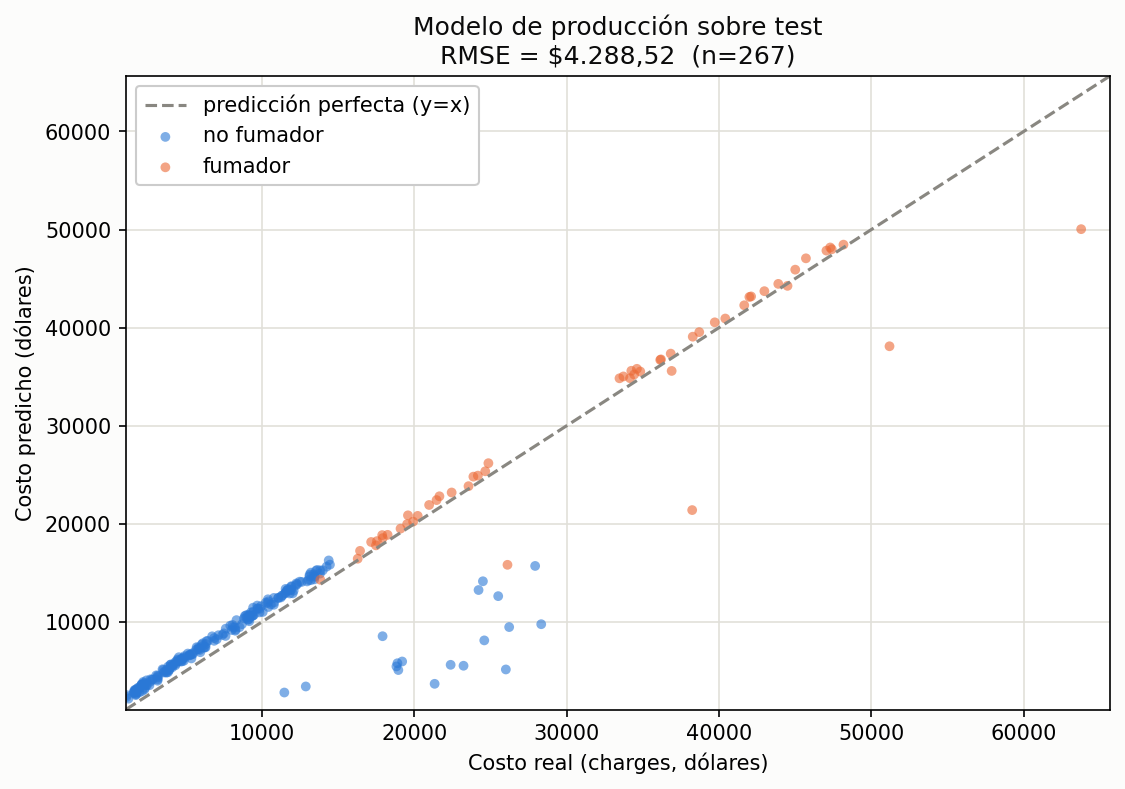
\includegraphics[width=0.72\textwidth]{05-predicho-vs-real.png}}{%
  \fbox{\parbox{0.72\textwidth}{\centering\vspace{1em}Figura pendiente: se genera al
  correr \texttt{python -m src.evaluar\_test}.\vspace{1em}}}}
\caption{Predicho contra real sobre el conjunto de test. El modelo acierta con precisión en la
mayoría barata (nube azul sobre la diagonal) y se dispersa en los casos caros, que son casi
todos fumadores: es la asimetría del error que la segunda advertencia menciona.}
\end{figure}

\subsection{Los once coeficientes del modelo de producción}

\begin{table}[H]
\centering
\caption{El modelo entero. Son las once características de grado 1, sin penalización: no hay
selección que reportar porque no hay nada de más que apagar. Los coeficientes están sobre
características estandarizadas, así que sus magnitudes son comparables entre sí ---con una
salvedad importante: \texttt{age} y \texttt{edad\_al\_cuadrado} son función determinista una de
la otra, y lo mismo \texttt{bmi}, \texttt{smoker=yes} y \texttt{bmi\_si\_fuma} entre sí. Dentro
de cada uno de esos grupos colineales el coeficiente individual no se interpreta solo: hay que
leer el grupo completo (ver \emph{Advertencia de interpretabilidad}, más arriba).}
\begin{tabular}{lr}
\toprule
\textbf{Característica} & \textbf{Coeficiente} \\
\midrule
\texttt{bmi\_si\_fuma}       & $\mathbf{5236{,}99}$ \\
\texttt{fumador\_obeso}      & $4891{,}83$ \\
\texttt{edad\_al\_cuadrado}  & $3749{,}13$ \\
\texttt{smoker=yes}          & $1161{,}22$ \\
\texttt{children}            & $815{,}02$ \\
\texttt{region=southwest}    & $-498{,}36$ \\
\texttt{region=southeast}    & $-424{,}86$ \\
\texttt{sex=male}            & $-218{,}32$ \\
\texttt{region=northwest}    & $-142{,}53$ \\
\texttt{bmi}                 & $111{,}20$ \\
\texttt{age}                 & $45{,}10$ \\
\bottomrule
\end{tabular}
\end{table}

\paragraph{El hallazgo.} \textbf{Los tres coeficientes más grandes del modelo son, en orden, las
tres características derivadas}: \texttt{bmi\_si\_fuma} (5236,99), \texttt{fumador\_obeso}
(4891,83) y \texttt{edad\_al\_cuadrado} (3749,13), las tres por encima de \texttt{smoker=yes}
(1161,22), que en el modelo original era el término dominante. El modelo dice, leído en orden:
la pendiente del bmi entre fumadores es lo que más pesa; ser fumador \emph{y} obeso suma otro
tanto encima; la curvatura de la edad importa casi tanto como las dos anteriores; y recién
después aparece el efecto de fumar por sí solo, ya reducido porque buena parte de lo que hacía
antes ---la pendiente distinta según el bmi--- ahora lo explica \texttt{bmi\_si\_fuma} de forma
directa. Es el mismo fenómeno que la advertencia de interpretabilidad ya anticipaba: las
características derivadas no compiten con las originales por espacio en el modelo, les
\emph{absorben} el efecto.

Vale la pena contrastarlo con lo que hacía el modelo anterior a D-23. Ahí la penalización $L_1$
dejaba vivas 10 de 44 características y el término \texttt{bmi*smoker=yes} quedaba tercero en
magnitud, por encima de \texttt{bmi} sola: \emph{el Lasso había encontrado la interacción por su
cuenta}, sin que nadie se la indicara. Ese resultado sigue en pie y es una buena demostración de
para qué sirve $L_1$ ---pero encontraba la interacción en la única forma que su espacio de
características le permitía, como un cambio de pendiente. El análisis exploratorio mostró que la
forma correcta era un escalón, y darle esa columna directamente al modelo resultó valer más que
toda la maquinaria que la aproximaba.

\begin{figure}[H]
\centering
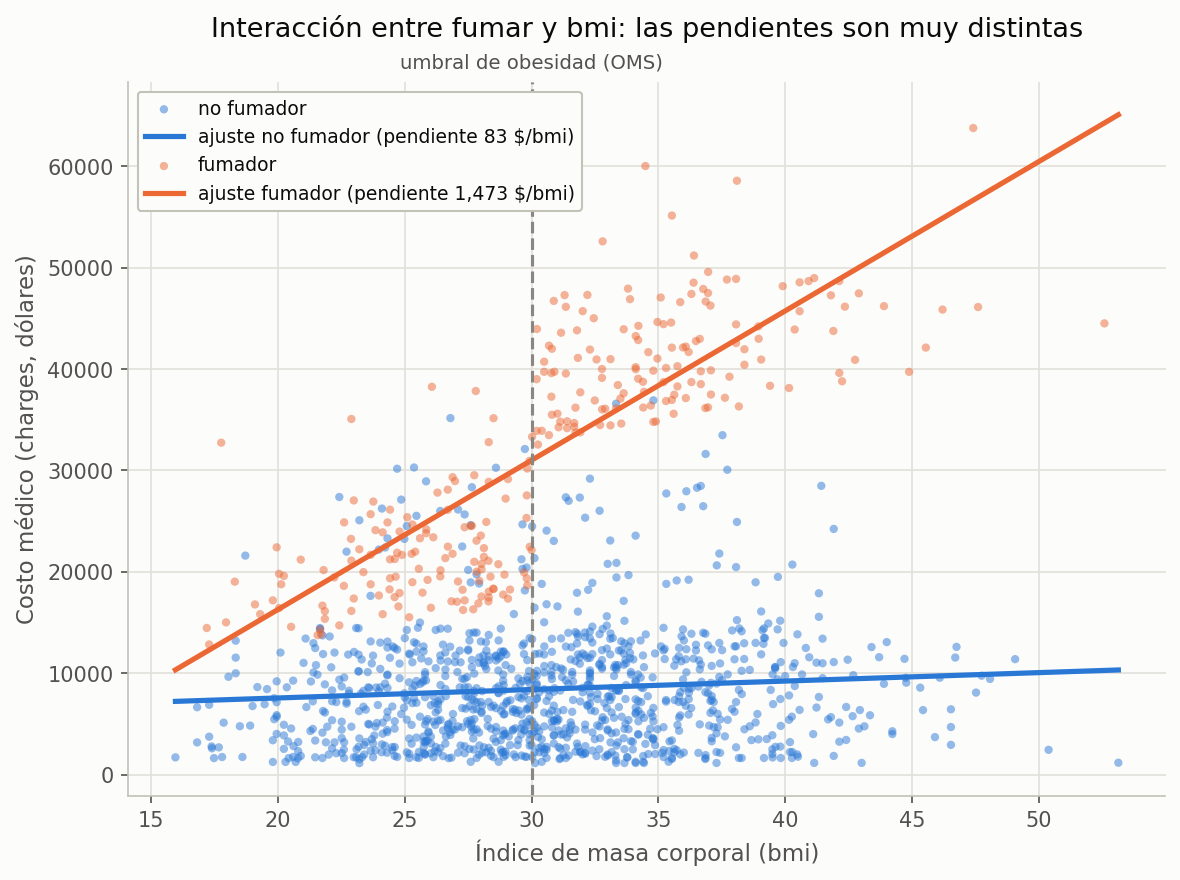
\includegraphics[width=0.82\textwidth]{03-interaccion-smoker-bmi.png}
\caption{La interacción, cuantificada. Ajustando una recta por grupo, la pendiente es de
\textbf{83 dólares por unidad de BMI} entre los no fumadores y de \textbf{1473} entre los
fumadores: un factor de \textbf{17,7}. Un modelo puramente aditivo sobre las variables crudas no
puede representar esa diferencia; \texttt{fumador\_obeso} sí, y con un solo coeficiente.}
\end{figure}

\subsection{Sensibilidad al número de folds: ¿y si $k$ no fuera 5?}
\label{sec:sensibilidad-k}

Toda la sección anterior descansa sobre $k=5$. Conviene preguntarse cuánto de la respuesta es del
modelo y cuánto es de esa elección.

\begin{center}
\fbox{\parbox{0.95\textwidth}{\small\vspace{2pt}
\textbf{Estado de esta sección tras D-27/D-28.} El barrido controlado con la configuración de
producción fija ---la figura \ref{fig:sensibilidad-k} y todo lo que se dice sobre ella--- está
\textbf{rehecho} con las once características vigentes (cuesta minutos, no horas:
\texttt{resultados/sensibilidad\_k.csv}). La \textbf{selección completa} ---las 19
configuraciones, en $k=5$, $10$ y $20$, la tabla de más abajo--- \textbf{no}: correrla sobre las
1364 columnas del grado 4 cuesta unas 5 horas por cada valor de $k$, y no se volvió a pagar ese
costo porque la corrida más reciente disponible ---con el pipeline de \textbf{nueve}
características, posterior a D-23 y anterior a D-27/D-28--- ya mostraba que el modelo de
producción no se movía con $k$; queda preservada en \texttt{resultados/sensibilidad\_k.json} y,
con el mismo contenido bajo otro nombre desde que D-27/D-28 la dejó atrás, en
\texttt{sensibilidad\_k\_previo\_d27.json}. La tabla de más abajo es todavía una generación
anterior a esa: el pipeline de \textbf{ocho} características, previo a D-23, preservado en
\texttt{sensibilidad\_k\_previo\_d23.json}. Su conclusión ---el modelo de producción no se mueve
con $k$--- es la que las dos corridas posteriores vinieron a confirmar, no a poner en
duda.\vspace{2pt}}}
\end{center}

\paragraph{Nada de esto vuelve a tocar el test.} El módulo \texttt{src/sensibilidad\_k.py} rehace
el mismo split con la misma semilla y descarta \texttt{idx\_test} sin usarlo: todo ocurre dentro
de las 1070 filas de train. No re-evalúa el test ---lo que violaría la doctrina de la sección
anterior--- sino que mide cuán estable es un procedimiento de selección que ya se ejecutó.

\paragraph{La pregunta que importa: ¿cambia el modelo elegido?} Se repitió la selección completa
---las 19 configuraciones, la regla de 1 error estándar, el criterio de parsimonia--- con $k=5$,
$10$ y $20$.

\begin{table}[H]
\centering
\small
\caption{La selección del punto 5, recalculada con tres valores de $k$ ---\emph{en el pipeline
anterior a D-23, ocho características}, ver el recuadro---. La última fila es la respuesta: el
modelo de producción no se mueve.}
\begin{tabular}{@{}l ccc@{}}
\toprule
 & $k=5$ & $k=10$ & $k=20$ \\
\midrule
Filas de entrenamiento por fold      & 856 & 963 & 1016 \\
Ganador crudo de la CV               & lasso g4, $\lambda$=286,4 & lasso g4, $\lambda$=95,5 & lasso g4, $\lambda$=95,5 \\
RMSE de validación del ganador       & 4920,0 & 4833,2 & 4744,8 \\
Error estándar $\sigma/\sqrt{k}$     & 100,3 & 229,2 & 230,7 \\
Configuraciones dentro de 1 ES       & 8 & 9 & 9 \\
\midrule
\textbf{Producción (regla de 1 ES)}  & \multicolumn{3}{c}{\destacado{lasso grado 2, $\lambda = 286{,}37$ --- en los tres}} \\
\bottomrule
\end{tabular}
\end{table}

\destacado{El modelo de producción es idéntico en los tres casos.} La respuesta del punto 5 no es
un artefacto de haber puesto 5.

Dos cosas sí se mueven, y conviene declararlas. El \textbf{ganador crudo} cambia de $\lambda$, y
el que queda solo es $k=5$: con 856 filas por fold el grado 4 necesita más regularización que con
963 o 1016. Es el sesgo de la curva de aprendizaje, medible y no teórico ---aunque irrelevante
para lo que se entrega, porque el ganador crudo no es el modelo de producción---. Y la
\textbf{banda de 1 ES se ensancha}: de 8 a 9 configuraciones indistinguibles.

\paragraph{Qué le pasa a los dos números que reporta este informe.} Fijando la configuración de
producción y variando sólo $k$ ---para que la única causa de las diferencias sea $k$--- aparecen
dos hallazgos distintos, y el primero corrige una lectura tentadora.

\begin{figure}[H]
\centering
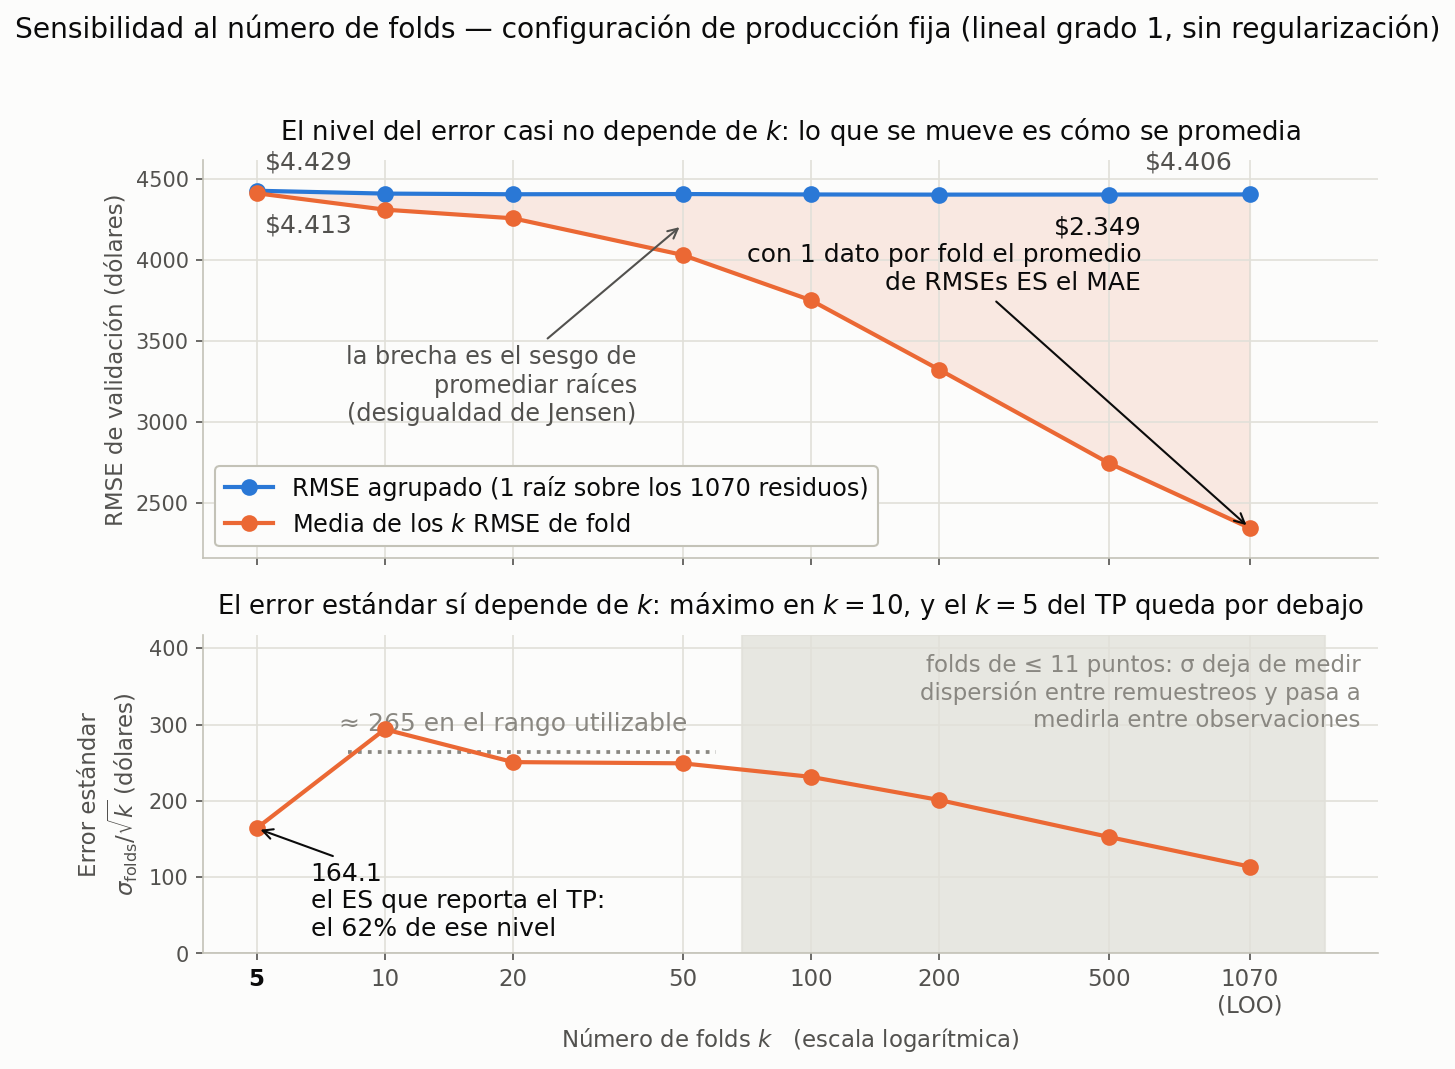
\includegraphics[width=\textwidth]{06-sensibilidad-k.png}
\caption{Sensibilidad al número de folds, con la configuración de producción fija (lineal grado 1,
sin regularizar, once características). Los ocho valores de $k$ dejan folds de 214, 107, 54, 21,
11, 5, 2 y 1 punto. \textbf{Arriba:} el nivel del error casi no depende de $k$ ---la curva
agrupada va de 4428,7 a 4405,9, un 0,51\,\%---; lo que se desploma es la \emph{forma de
promediarlo}, y el área sombreada entre las dos curvas es ese sesgo. \textbf{Abajo:} el error
estándar sí depende de $k$, con un máximo de 293,9 en $k=10$ y una caída posterior; el $k=5$ del
informe vale 164,1. La banda gris marca dónde los folds son tan chicos que $\sigma$ deja de medir
dispersión entre remuestreos.}
\label{fig:sensibilidad-k}
\end{figure}

\textbf{Primero: la caída del RMSE es un artefacto de la métrica, no del modelo.} El pipeline
reporta la \emph{media de los $k$ RMSE de fold}, y esa media baja $2064{,}9$ dólares
($4413{,}4 \rightarrow 2348{,}5$) al ir de $k=5$ a LOO. Es tentador leerlo como que $k=5$ es
fuertemente pesimista, pero no lo es: la raíz es cóncava, así que por desigualdad de Jensen
\begin{equation}
\operatorname{media}_i \sqrt{\mathrm{ECM}_i} \;<\; \sqrt{\operatorname{media}_i \mathrm{ECM}_i},
\end{equation}
con una brecha que crece a medida que los folds se achican. Calculando en cambio el \textbf{RMSE
agrupado} ---una sola raíz sobre los 1070 residuos \emph{out-of-fold} juntos, que no tiene ese
sesgo--- el error va de $4428{,}7$ a $4405{,}9$: \destacado{22,8 dólares, un 0,51\,\%}, y agotados
ya en $k=20$. El sesgo pesimista real de $k=5$ es despreciable.

Ese mismo fenómeno, llevado al extremo, es lo que vuelve inservible a \emph{leave-one-out} con
este pipeline: con un solo dato por fold $\mathrm{RMSE}_i = |y_i - \hat y_i|$, y el promedio de
los $k$ RMSE \textbf{es literalmente el MAE} ($2348{,}5$) ---un 46,7\,\% por debajo del RMSE
agrupado del mismo $k$ ($4405{,}9$), y no comparable contra el RMSE de test de este informe---.
LOO no es «más validación»: rompe la métrica en silencio, además de exigir ajustar cada
configuración 1070 veces en lugar de 5.

\textbf{Segundo: el error estándar tiene un único pico, en $k=10$, y no una meseta.} Midiendo la
grilla densa ---$k=5,10,20,50,100,200,500,1070$--- el ES sube de $164{,}1$ en $k=5$ a un máximo de
$293{,}9$ en $k=10$, y de ahí cae de forma monótona: $250{,}9$ / $249{,}3$ / $231{,}6$ / $201{,}3$
/ $152{,}8$ / $114{,}0$ hasta LOO. No hay meseta entre $k=10$ y $k=50$: el pico está en un solo
punto y la curva ya está bajando en $k=20$.

El mecanismo se verifica contra los propios datos: si $\sigma$ (el desvío del RMSE entre folds)
creciera exactamente como $\sqrt{k}$, el ES sería constante. De $k=5$ a $10$, $\sigma$ salta
\destacado{$2{,}53\times$} ($367{,}0 \rightarrow 929{,}5$) donde $\sqrt{k}$ predice sólo
$1{,}41\times$ ---la $\sigma$ de $k=5$ está estimada con \emph{cinco} números y
\texttt{ddof=0}, un estimador ruidoso y sesgado hacia abajo---, y ese exceso es lo que empuja el
ES hacia arriba. Pasado el pico la relación se invierte: $\sigma$ sigue creciendo, pero en
promedio más lento que $\sqrt{k}$ (de $k=500$ a LOO salta $1{,}09\times$ donde $\sqrt{k}$ predice
$1{,}46\times$), porque con folds de 2 o 1 punto $\sigma$ deja de medir variabilidad entre
remuestreos y empieza a saturar contra la dispersión de los residuos individuales ---la banda gris
de la figura~\ref{fig:sensibilidad-k}.

Las razones son dato medido; que las causas sean esas dos es la lectura más razonable del patrón,
no una descomposición formal de la varianza. Lo que sí queda establecido es que el pico,
$293{,}9$ en $k=10$, es \destacado{$1{,}79$ veces} el $164{,}1$ que la regla de 1 ES usó en la
selección del punto 5.

\paragraph{Consecuencia.} No se cambia el esquema: el modelo de producción no se mueve (lo mostraron
las dos corridas anteriores para $k=5,10,20$ ---la tabla de más arriba, con ocho características,
y la corrida de nueve preservada en \texttt{sensibilidad\_k.json}---, y no hay motivo para
esperar algo distinto con las once vigentes), el nivel del error no depende de $k$ una vez
corregida la forma de promediar, y el test ---evaluado \textbf{tres} veces sobre la misma
partición, según D-26 y D-29--- no se vuelve a tocar en este barrido. Lo que cambia es lo que
este informe \emph{declara}: el error estándar de la selección podría llegar a ser
\destacado{$1{,}79$ veces} el $164{,}1$ usado en el punto 5, no una meseta plana entre $200$ y
$250$. Eso no debilita la elección del modelo simple ---la refuerza: con un ES más ancho hay más
configuraciones estadísticamente indistinguibles del mejor, no menos---.

\subsection{Dónde vive el error que queda}
\label{sec:diagnostico-residuos}

D-23, D-27 y D-28 bajaron el RMSE de test de 4.739,33 a \rmsetestproduccion{} dólares. La
pregunta que sigue es si se puede bajar más, y con qué. \texttt{D-30} contesta con un
diagnóstico \emph{out-of-fold} sobre train: para cada una de las 1070 filas, la predicción sale
de un modelo que \textbf{no la vio} durante el ajuste ---el mismo esquema de 5 folds del punto 4,
pero guardando el residuo de cada fila en vez de sólo el RMSE agregado--- en
\texttt{src/diagnostico\_residuos.py} (\texttt{resultados/diagnostico\_residuos.csv}). No toca
\texttt{X\_test}: es un diagnóstico sobre train, no una evaluación más del modelo.

\paragraph{El error no está repartido.}

\begin{table}[H]
\centering
\caption{Concentración del error cuadrático (SSE) sobre las filas de train, ordenadas de mayor a
menor residuo.}
\begin{tabular}{lrr}
\toprule
\textbf{Fracción de filas} & \textbf{Filas} & \textbf{\% del SSE total} \\
\midrule
1\,\%  & 10  & $23{,}53$\,\% \\
5\,\%  & 53  & $75{,}38$\,\% \\
10\,\% & 107 & $91{,}54$\,\% \\
\bottomrule
\end{tabular}
\end{table}

Diez personas ---el 1\,\% del train--- explican casi una cuarta parte del error cuadrático
total. El 5\,\% explica tres cuartas partes. El modelo no está mal en todos lados por igual: está
muy bien en la enorme mayoría de las filas y muy mal en un núcleo chico.

\paragraph{Por población.}

\begin{table}[H]
\centering
\caption{Reparto del error cuadrático por población. El error se concentra en los
\textbf{no fumadores}, no en los fumadores obesos que motivaron \texttt{fumador\_obeso} (D-23).}
\begin{tabular}{lrrr}
\toprule
\textbf{Población} & \textbf{$n$} & \textbf{RMSE} & \textbf{\% del SSE total} \\
\midrule
No fumadores               & 850 & 4615 & $\mathbf{86{,}3}$\,\% \\
Fumadores, bmi $\leq 30$   & 105 & 3407 & $5{,}8$\,\% \\
Fumadores, bmi $> 30$      & 115 & 3804 & $7{,}9$\,\% \\
\bottomrule
\end{tabular}
\end{table}

Es un resultado que a primera vista sorprende: adentro de ``no fumadores'' hay, otra vez, una
subpoblación de facto que ni \texttt{fumador\_obeso} ni \texttt{bmi\_si\_fuma} distinguen, porque
las dos características derivadas están construidas alrededor de \texttt{smoker=yes}.

\paragraph{El núcleo: 28 personas que ninguna columna distingue.} Filtrando a los no fumadores
con \texttt{charges} $>25.000$ ---28 filas, $2{,}6$\,\% del train--- ese grupo aporta el
\destacado{$41{,}9$\,\% del error cuadrático total}, y el modelo los \destacado{subestima en
promedio 17.378 dólares}. Es, con amplio margen, el bloque más grande de error de todo el
dataset.

Y no se los puede identificar con las columnas disponibles:

\begin{table}[H]
\centering
\caption{Perfil de las 28 personas del núcleo contra el resto de los no fumadores. La única
diferencia que se nota es la edad.}
\begin{tabular}{lrr}
\toprule
\textbf{Variable} & \textbf{Estas 28 personas} & \textbf{Resto de los no fumadores} \\
\midrule
age (media)      & $\mathbf{50{,}79}$ & $39{,}11$ \\
bmi (media)      & $31{,}23$ & $30{,}69$ \\
children (media) & $1{,}39$ & $1{,}10$ \\
sex              & 54\,\% F / 46\,\% M & 51\,\% F / 49\,\% M \\
region           & pareja a la del resto & pareja a la del resto \\
\bottomrule
\end{tabular}
\end{table}

Bmi, \texttt{children}, sexo y región son prácticamente el mismo perfil que el resto de los no
fumadores; sólo la edad se separa (50,8 contra 39,1), y no alcanza para aislar al grupo. Ninguna
combinación de las columnas originales ---ni siquiera sumando las tres características
derivadas del pipeline vigente--- lo separa del resto antes de ver \texttt{charges}.

\paragraph{Conclusión: error irreducible con este dataset.} Ese $\sim$42\,\% del error cuadrático
\textbf{no es falta de capacidad del modelo}: falta la variable que explica el gasto ---una
patología, una cirugía, una condición preexistente--- y esa variable no está en el CSV. Ninguna
familia de modelos, por más flexible que sea, puede recuperar una señal que no está en las
columnas de entrada; agregarle grados de libertad ahí sólo memoriza ruido, que es exactamente el
sobreajuste que documenta el punto 4 en los grados 3 y 4.

Esto se verifica contra el propio historial de este trabajo: el diagnóstico se corrió
\textbf{después} de D-27 y D-28, o sea sobre el pipeline ya mejorado, y el núcleo sigue
concentrando el $41{,}9$\,\% del error. Las dos características nuevas bajaron el RMSE de test
450,81 dólares desde el pipeline de ocho, pero no tocaron este núcleo: es la evidencia de que ese $\sim$42\,\% es un
piso, no una debilidad de esta familia de modelos en particular. \destacado{Para bajar ese tramo
del error hace falta otra variable, no otro modelo.}

% =====================================================================
\section{Limitaciones}
% =====================================================================

\begin{itemize}
  \item \textbf{Colinealidad en grados altos.} En grado 4, el 68,0\,\% de las 1364 columnas son
        redundantes (rango efectivo 436). Hay tres causas. Primera: una dummy binaria elevada a
        una potencia sigue teniendo sólo dos valores posibles, así que es una función afín
        exacta de la dummy original ---por ejemplo
        $\texttt{smoker=yes}^2 = 1{,}456866 \cdot \texttt{smoker=yes} + 1{,}0$, con un residuo
        de $1{,}5\times10^{-14}$, matemáticamente exacto salvo error de punto flotante---.
        Segunda: el producto de dos dummies del mismo one-hot cae dentro del espacio generado
        por las dummies individuales más la constante, porque 3 dummies y una constante ya
        generan todas las funciones posibles sobre las 4 regiones. Tercera, y nueva desde
        D-27/D-28: la expansión polinómica \textbf{duplica exactamente} a las dos características
        derivadas a partir de grado 2 ---$\texttt{age}^2$ coincide con
        \texttt{edad\_al\_cuadrado}, y $\texttt{bmi}\cdot\texttt{smoker=yes}$ con
        \texttt{bmi\_si\_fuma}---, y es la causa de que la redundancia suba del 59,7\,\% (sin las
        dos derivadas) al 68,0\,\% actual, y de que cuatro configuraciones no converjan en vez de
        dos. En grado 1, el de producción, no hay duplicación: las once columnas son de rango
        completo.

        Conviene aclarar que ese producto \textbf{no es idénticamente cero}: lo sería en la
        codificación cruda 0/1, pero como el pipeline estandariza antes de expandir, cada dummy
        toma valores distintos de 0 y 1 y el producto también. Sigue siendo redundante, por la
        segunda razón, no por ser nulo. La consecuencia práctica es que \textbf{dentro de un
        grupo colineal el reparto de coeficientes es arbitrario}: no se pueden interpretar de a
        uno cuando el grado es alto.

  \item \textbf{Una sola partición train/test, con una sola semilla.} El RMSE de test reportado
        tiene varianza asociada a qué filas cayeron del lado de test, que este trabajo no midió.
        Repetir el split con otra semilla daría un número distinto, presumiblemente cercano pero
        no idéntico.

  \item \textbf{El test se evaluó tres veces} (D-26, D-29). La primera con el modelo del
        pipeline anterior a D-23, la segunda con el modelo corregido tras el análisis
        exploratorio de la Clase 3 (\texttt{fumador\_obeso}), la tercera con
        \texttt{edad\_al\_cuadrado} y \texttt{bmi\_si\_fuma} (D-27, D-28). Las tres elecciones se
        hicieron íntegramente con validación cruzada sobre \texttt{train} ---ningún diagnóstico
        de \texttt{src/evidencia\_features.py} ni de \texttt{src/diagnostico\_residuos.py}
        construye \texttt{X\_test}---, y este informe publica \emph{los tres} números de test, no
        sólo el favorable: es la única forma de que el lector verifique que no se eligió mirando
        el resultado. El costo es real, no sólo nominal: reutilizar la misma partición se aparta
        del protocolo ideal, y cada evaluación extra erosiona un poco su independencia. Se acepta
        la desviación porque comparar las tres etapas sobre las mismas filas vale más que pedir
        una partición nueva cada vez ---no porque el costo sea nulo.

  \item \textbf{El umbral de \texttt{fumador\_obeso} no se validó como hiperparámetro.} Se tomó
        el de la OMS, que es externo al dataset. El barrido de umbrales de D-23 lo confirma
        \emph{a posteriori}, pero si el corte se hubiera elegido por ese barrido sería un
        hiperparámetro ajustado contra validación y el RMSE de validación quedaría sesgado a la
        baja. No es el caso, y la distinción importa.

  \item \textbf{El dataset es simulado.} Proviene de estadísticas demográficas ---el origen es
        el dataset del libro de Lantz--- y no del registro de una aseguradora real, así que las
        relaciones que el modelo aprendió reflejan cómo se construyó la simulación.

  \item \textbf{El RMSE penaliza el error al cuadrado}, con lo cual la métrica está dominada
        por los casos caros. Un modelo puede tener un RMSE relativamente bueno y aun así errar
        de forma proporcionalmente grande en los casos baratos.
\end{itemize}

% =====================================================================
\section{Guion de la presentación (10 minutos)}
% =====================================================================

\begin{table}[H]
\centering
\small
\caption{Reparto del tiempo. La introducción teórica y el punto 5 son lo que más se evalúa.}
\begin{tabular}{@{}c p{9.6cm} p{3.3cm}@{}}
\toprule
\textbf{Min.} & \textbf{Qué se dice} & \textbf{Figura} \\
\midrule
0--1 & Dataset (\texttt{insurance.csv}, 1338 filas) y la pregunta del TP: predecir \texttt{charges} y elegir un modelo defendible, no sólo el de menor error. & --- \\
1--3 & Introducción teórica: por qué train no alcanza, qué rol cumple cada conjunto, por qué el test se toca una sola vez, y qué gana la validación cruzada frente a un único split. & --- \\
3--4 & Punto 1: por qué se conservan los 139 outliers (97,8\,\% fumadores) y por qué IQR y no z-score. & \texttt{04-outliers} \\
4--5 & Puntos 2 y 3: el pipeline y por qué la regresión polinómica sigue siendo lineal en los parámetros. & --- \\
5--7 & Punto 4: las curvas por grado, dónde aparece el sobreajuste (la brecha de 61,8 a 84.537,9, el desvío de $\pm$367 a $\pm$47.000) y cómo Lasso lo corrige. & \texttt{01-curvas}, \texttt{02-camino} \\
7--9 & Punto 5, el núcleo: por qué el lineal grado 1 gana la CV siendo además el más simple del espacio, por qué 7 de las 15 son indistinguibles y confirman la misma elección, y el RMSE prometido, con el sesgo del mínimo. & \texttt{una-es} \\
9--10 & Limitaciones y cierre. & --- \\
\bottomrule
\end{tabular}
\end{table}

% =====================================================================
\appendix
\section{Reproducibilidad}
% =====================================================================

El repositorio corre con Python 3.10 o superior y solamente \texttt{numpy}, \texttt{pandas} y
\texttt{matplotlib}. No usa \texttt{scikit-learn} ni \texttt{pytest}.

\begin{table}[H]
\centering
\begin{tabular}{@{}l l@{}}
\toprule
\textbf{Comando} & \textbf{Qué hace} \\
\midrule
\texttt{python -m src.datos}       & Punto 1: análisis exploratorio \\
\texttt{python -m src.experimentos}& Puntos 2 a 5 (unos 27 minutos) \\
\texttt{python -m src.evidencia\_features} & La evidencia numérica de D-23, D-24, D-25, D-27 y D-28 \\
\texttt{python -m src.diagnostico\_residuos} & El diagnóstico de residuos y el error irreducible de D-30 \\
\texttt{python -m src.graficos}    & Genera las figuras de este informe \\
\texttt{python -m src.tablas}      & Regenera las tablas del punto 4 desde los CSV \\
\texttt{python -m src.sensibilidad\_k} & Barrido de $k$ de la sección \ref{sec:sensibilidad-k} (parte B, minutos; parte A completa, $\sim$5 h con el pipeline actual de 1364 columnas en grado 4) \\
\texttt{python -m tests.test\_validacion} & Suite del módulo de partición y métricas \\
\texttt{python -m tests.test\_preproceso} & Suite de codificación, escalado y expansión \\
\texttt{python -m tests.test\_modelos}    & Suite de los modelos \\
\texttt{python -m tests.test\_paleta}     & La paleta de las figuras, bajo simulación de daltonismo \\
\bottomrule
\end{tabular}
\end{table}

% sloppypar: el párrafo es casi todo \texttt{} con guiones bajos, que TeX no puede
% dividir; sin aflojar el espaciado entre palabras se desborda el margen.
\begin{sloppypar}
Los resultados están versionados en \texttt{resultados/} (\texttt{cv\_lineal.csv},
\texttt{cv\_lasso.csv}, \texttt{modelo\_elegido.json}, \texttt{evaluacion\_test.json},
\texttt{evidencia\_features.csv}, \texttt{diagnostico\_residuos.csv}, \texttt{sensibilidad\_k.json},
\texttt{sensibilidad\_k.csv}, \texttt{sensibilidad\_k\_previo\_d23.json},
\texttt{sensibilidad\_k\_previo\_d27.json} y \texttt{evaluacion\_test\_previo\_d27.json}), junto
con la salida completa de la corrida en \texttt{informe/salida-seleccion.txt}, de modo que no hace
falta correr nada para verificar los números de este informe. Las decisiones metodológicas están
numeradas y justificadas una por una en \texttt{DECISIONES.md}.
\end{sloppypar}

\paragraph{Procedencia del dataset.}
El archivo se descargó del enlace que da el enunciado
(\texttt{kaggle.com/datasets/mirichoi0218/insurance}) y se verificó que la copia usada es
byte a byte idéntica al original publicado:

\begin{center}
\texttt{\footnotesize SHA256 = 388eff679557d08ac19f463d025de5e0b4adc482537c8456d19934d78621fd47}
\end{center}

\end{document}
